\documentclass[UTF8,12pt]{article}
\usepackage{amssymb,amsfonts,amsmath,amsthm}

\usepackage{xeCJK}
\xeCJKsetup{AutoFallBack=true}
\usepackage{indentfirst}
\setlength{\parindent}{2em}

\renewcommand{\baselinestretch}{1.5}
\usepackage{xcolor}%colorhttps://cn.overleaf.com/project/5fcf7d918500b668a1d2395d
\usepackage{graphicx} %fig
\usepackage[normalem]{ulem}%underline
%建议你使⽤ ulem 宏包下
%的 uline 命令代替,它还⽀持换⾏⽂本。
%需要注意的是, ulem 宏包重定义了\emph命令, 使得原来的加斜强调变成
%了下划线、原来的两次强调就取消强调变成了两次强调就双下划线。通过宏包的
%normalem 选项可以取消这个更改: \usepackage[normalem]{ulem}。



\usepackage[a4paper]{geometry}
\geometry{
    tmargin=2cm,
    bmargin=2cm,
    lmargin=2cm,
    rmargin=2cm
}

%\usepackage[colorlinks,bookmarksopen=true,bookmarksnumbered=true]{hyperref}%超链接
% 由于它经常与其他宏包冲突,⼀般把它放在导⾔区的最后。
\title{流体力学复习笔记-2020}
\author{王洁峰}
\date{2020年11月8日}


\begin{document}
    \maketitle
    
    \newpage\tableofcontents\newpage
    
\section{绪论、数理基础}
牛顿内摩擦定律:\emph{流体的内摩擦力大小与
流体性质有关,与流体速度变化梯度和接触面积成正比。}
\begin{align*}
    F = \mu A \frac{du}{dy}
\end{align*}
F,内摩擦力,粘性力,与法向速度梯度有关,存在相对运动时产生,
只能减缓,不能阻止。没有粘性($\mu = 0$)的流体,即\emph{理想流体}。

满足上述牛顿内摩擦定律的流体称为\emph{牛顿流体},否则为非牛顿流体。

在流体力学中,描述流体运动的观点有两种:拉格朗日方法、欧拉方法。
\begin{description}
    \item[拉格朗日方法] 着眼于流体质点,描述每(某)个质点自始至终的运动过程
    \item[欧拉方法] 着眼于空间场,描述每(某)个空间点流体随时间变化的过程 
\end{description}

注意的是:\emph{拉格朗日描述}中的$t$是个变量,不变的是标记流体质点的$a,b,c$
描述了随时间某个以$a,b,c$确定的质点随时间是如何变化的。
\emph{欧拉描述}描述的某一个时刻,因此公式里往往没有$t$,如果有也是个定值,变量是$x,y,z$,
描述了随着空间坐标的变化,某个量是如何变化的。

场论:\emph{(不管是标量场,还是矢量场都是{\color{red}欧拉描述吧?})}

场:空间区域内的(矢量、标量)函数称为\emph{场}。
在场内定义的(矢量、标量)函数通常是时间$t$和空间$\vec r:x,y,z$的函数,
比如说:

\begin{align*}
    \varphi(\vec r,t) = \varphi (x,y,z,t)\\
    \vec a = \vec a (\vec r,t) = \vec a(x,y,z,t)
\end{align*}

下面介绍的\emph{均匀场}和\emph{定常场},
似乎与后面第二章的\emph{不可压缩流体
、均质流体、均质不可压缩流体、定常、非定常}有些关系,需要{\color{red} 抽空问下老师}。

\begin{description}
    \item[均匀场] 如果同一时刻各点函数值是相等的,因此坐标就无所谓了,
    所以$\varphi (x,y,z,t)$就简化为了$\varphi (t)$,同理,
    $\vec a(x,y,z,t)$简化为了$\vec a(t)$
    \item[定常场] 如果场内函数值不依赖时间,即不随时间变化,为\emph{定常场}
    ,跟时间没关系说白了就是把t去掉就行,于是简化为了$\varphi (\vec r), \vec a(\vec r)$
\end{description}

小结:均匀场和定常场跟矢量场还是标量场无关,不是一个维度的评判标准。
不管是标量场还是矢量场,应该都是需要固定个时间才知道某个时刻的状况,即
N维的状况,我觉得还是都还是\emph{欧拉}的描述。{\color{red} 对否?}

\emph{梯度}

梯度就是最大的方向导数,沿着等位线法向方向n的方向导数是最大的。
然后最大的这个方向导数(即梯度,方向是n),往任意方向的投影
(在任意方向上的投影)等于该方向上的方向导数。

\begin{center}
    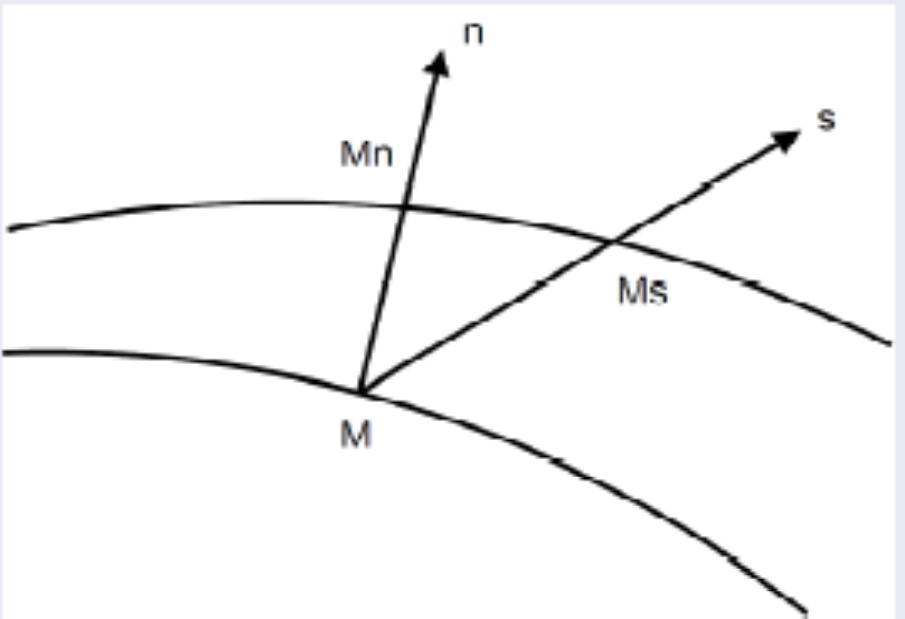
\includegraphics[width=0.5\linewidth]{img/tidu.png}
\end{center}

梯度性质
\begin{itemize}
    \item 标量场不均匀的量度 (实际上矢量场也能求梯度)
    \item 梯度方向与等位线的法向方向重合,指向$\varphi$增长的方向,
    大小是n方向上的方向导数$\frac{\partial \varphi}{\partial n}$
    \item 梯度方向上是函数$\varphi$变化最快的方向,梯度在任何方向s
    上投影等于该方向上的方向导数$\frac{\partial \varphi}{\partial s} = \frac{\partial \varphi}{\partial n}cos(\vec n,\vec s) = \vec s \cdot grad \varphi$其中$\vec s$是方向向量(单位向量)
\end{itemize}

$grad \varphi = [\frac{\partial \varphi}{\partial x},\frac{\partial \varphi}{\partial y},\frac{\partial \varphi}{\partial z}]^{T}$

\emph{散度}

\begin{align*}
    div \vec a = \frac{\partial a_x}{\partial x} 
                + \frac{\partial a_y}{\partial y} 
                + \frac{\partial a_z}{\partial z}
\end{align*}

\newpage
散度有以下几个物理意义:

\begin{itemize}
    \item 流出为正,流入为负,散度表示通量的概念
    (不可压缩流体的总散度必为零)
    \item 流体单位体积的改变率
    \item 辐聚/辐散
\end{itemize}

$div \vec a = 0$称为无源场或者管式场,性质如下(可略吧)
\begin{itemize}
    \item 无源矢量$\vec a$通过矢量管的任意截面的通量相同
    \item 矢量管不能再场内发生或者终止,只能延伸至无穷,靠在区域的边界上
    或自成封闭管路
    \item 无源矢量$\vec a$经过一已知周线L的所有曲面S上通量都相等
\end{itemize}

\emph{旋度}
\begin{center}
    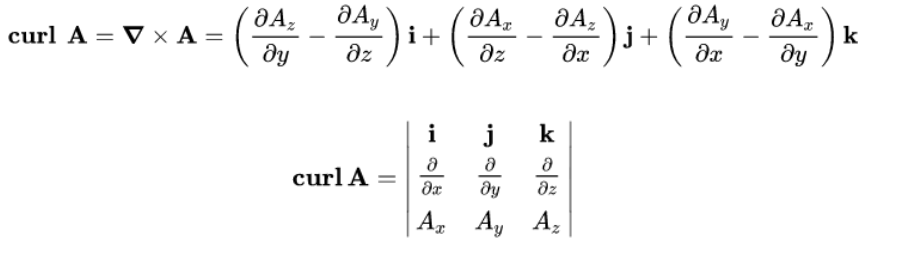
\includegraphics[width=.8\linewidth]{img/xuandu.png}
\end{center}

\emph{哈密顿算子}
\begin{align*}
    \bigtriangledown = \vec i \frac{\partial}{\partial x} 
                        + \vec j \frac{\partial}{\partial y}
                        + \vec k \frac{\partial}{\partial z}
\end{align*}
具有矢量和微分双重性质,(其实不就是求梯度吗?)
注意!他只对右边的变量发生微分作用。
\emph{这也是我在小测中经常做错的原因,有时候对左侧的也微分起来的了。}

\newpage
\section{流体运动学基础}
流体力学就是研究流体(一种连续介质)的宏观运动的力学分支。

{\color{cyan} 连续介质假设}
认为:真是流体所占有的空间可近似的看做由
\emph{流体质点(微团)}
连续地无间隙地充满的。

{\color{cyan} 流体质点(微团)}
指的是宏观上足够小而在微观上足够大的分子团。
    一方面,分子团的尺度与分子运动尺度相比大得多
,包含足够多的分子,是的个别分子进出不影响统计平均特性。
    另一方面相对宏观运动尺度足够小,使得分子团
在平均物理量在宏观运动尺度上可看成均匀不变的。

连续介质假设的前提是\emph{运动的宏观尺度要远远大于微观尺度}。
也就是研究对象宏观运动和物质结构微观尺度 
相当的时候,连续介质假设不再适用,比如在高孔稀薄大气里面的航天器。

这一章是流体运动学,在不考虑外力作用下,用数学和几何方法描述流体的
{\color{cyan} 平动、转动、变形}。

\subsection{流体运动描述方法、几何表述}

流体力学中,描述流体运动的观点和方法有两种:
\begin{description}
    \item[拉格朗日方法] 着眼于流体质点,设法描述出\uline{每个}质点自始至终的运动过程,即
    他们的位置和其他属性(如速度,加速度,温度,压强等)随时间变化的规律
    \item[欧拉方法] 着眼于空间点(场),设法在空间中的\uline{每一点}上描述出流体运动随时间
    的变化状况
\end{description}
其实上面说的真的做到了吗?没啊,拉格朗日说的\uline{每个}质点,欧拉说的每个空间点
其实只是分别用$(a,b,c)~or~(x,y,z)$来表示了,哦,这是未知的,这就代表了所有,有种
函数解析式的感觉了,但我/每个人直观的感受是-把它列举出来,一个一个的列举出来。

\subsection{拉格朗日方法}

要描述的物理量(空间位置、速度、加速度、密度、温度、压强等)
表示成为
初始位置坐标($t_0$时刻或$t=0$时候位置定为$(a,~b,~c)$)
和时间t的函数。

比如,描述的物理量是流体质点的位置随时间的变化
(流体质点的运动规律)可以表示为:
\begin{align*}
    \vec r = \vec r(a,~b,~c,~t)
\end{align*}
$\vec r$为矢径,上述公式在直角坐标下,分量表示形式是:
\begin{align*}
    x &= x(a,~b,~c,~t)\\
    y &= y(a,~b,~c,~t)\\
    z &= z(a,~b,~c,~t)
\end{align*}

每确定了一组$a,~b,~c$,就确定了一个流体质点的运动方程和轨迹。

拉格朗日描述中,速度$\vec v$是该质点矢径$\vec r$的时间变化率,
加速度$\vec a$是该质点速度$\vec v$的时间变化率,所以:
\begin{align*}
    \vec v(a,~b,~c,~t) &= \frac{\partial \vec r (a,~b,~c,~t)}{\partial t}\\
    \vec a(a,~b,~c,~t) &= \frac{\partial \vec v (a,~b,~c,~t)}{\partial t} = \frac{\partial ^2 \vec r (a,~b,~c,~t)}{\partial t^2}
\end{align*}

\emph{矢径}仅仅是质点标号(a,b,c)的函数,不是空间坐标的函数,
因此\emph{矢径}不是场\footnote{空间区域内定义的标量函数、矢量函数称为场}。

\subsection{欧拉方法}

\begin{description}
    \item[定常流动] 流动不随时间变化\emph{(这说的是速度场吧?}
\end{description}

对定常流动,欧拉表述的物理量不随时间变化。
\emph{定常流动不是指的是流动吗?那其描述的物理量难道不是速度吗?{\color{red} 还能有别的吗}}
\emph{另外,欧拉描述与拉格朗日描述所能描述的物理量应该没啥限制吧?都能
速度、加速度、密度、温度、压强吧?欧拉的话,矢量场 标量场应该都行,这些物理量
在拉格朗日描述里 不能叫场,只能叫拉格朗日所描述的物理量吧。还有拉格朗日描述的温度,压强
一旦求导,对时间求导有啥物理意义?}

欧拉描述函数的变量是空间位置a,b,c与时间t。
\begin{align*}
    \vec v = \vec v(\vec r,~t)
\end{align*}

在直角坐标系下:

\begin{align*}
    u &= u(x,~y,~z,~t)\\
    v &= v(x,~y,~z,~t)\\
    w &= w(x,~y,~z,~t)
\end{align*}

其中,$(x,~y,~z,~t)$称为欧拉变数,同样可以定义空间点上的
密度$\rho(\vec r,~t)$,压强$p(\vec r,t)$和温度$T(\vec r,t)$等。

上面说的这些是空间点$(x,y,z)$的函数,因此是场。比如,速度场是矢量场,
密度场、温度场是标量场。

均匀场:场内函数不依赖与空间坐标。定常场:场内函数不依赖时间t。

欧拉描述下,求导是全导数,以加速度(速度的求导)为例:
\begin{align*}
    \frac{d\vec v}{dt} = \frac{\partial \vec v}{\partial t} + (\vec v \cdot \bigtriangledown) \vec v
\end{align*}
\begin{description}
    \item[左手第一项] 随体导数 $\frac{d\vec v}{dt}$:流体质点的速度随时间的变化率,局地导数和位变导数的和,也称为物质导数
    \item[右手第一项] 局地导数 $\frac{\partial \vec v}{\partial t}$ 由于场的不定常性,引起的速度变化对质点加速度的贡献
    \item[右手第二项] 位变导数 $(\vec v \cdot \bigtriangledown) \vec v$由于场的不均匀性引起的速度变化对质点加速度的贡献,流体质点沿着轨迹L移动引起的速度变化
\end{description}

在欧拉描述下,随体导数分解成局地导数和位变导数对欧
拉描述的任何物理量(不管是矢量$\vec a$还是标量$\varphi$)都是成立的,即:
\begin{align*}
    \frac{d\varphi}{dt} &= \frac{\partial \varphi}{\partial t} + (\vec v \cdot \bigtriangledown) \varphi\\
    \frac{d\vec a}{dt} &= \frac{\partial \vec a}{\partial t} + (\vec v \cdot \bigtriangledown) \vec a
\end{align*}

质点的密度$\rho$在运动过程中不变的流体是不可压缩的流体,流体各点密度$\rho$都相等的流体称为均值流体
。
\subsection{拉格朗日-欧拉转换}
\subsubsection{拉格朗日2欧拉}

基本思路:
\begin{itemize}
    \item 已知的质点位置的拉格朗日描述,直接对时间t求导可以得到拉格朗日描述下的速度与加速度。
    \item 因为欧拉描述不能有a,b,c等常数,得替换掉,
    \item 替换方法是根据已知的位置方程,反解出a,b,c,
    \item 再代入拉格朗日描述下的速度、加速度,
    这样,拉格朗日描述就变成了欧拉描述。
\end{itemize}

\subsubsection{欧拉2拉格朗日}

基本思路:
\begin{itemize}
    \item 已知空间位置上的速度或者加速度,本身是矢径的一阶全导数/二阶全导数
    \item 积分上述一阶/二阶常微分方程,就得出了矢径的解(含x,y,z与t)
    \item 这时候代入$t=0$,令x,y,z = a,b,c求出未知的C,带回方程得出x,y,z = (a,b,c,t)的方程
    \item 根据已知条件,将已知条件改为拉格朗日方程
\end{itemize}

小结:{\color{cyan} 需要注意的是}-拉格朗日描述下:位置矢量$\rightarrow$速度矢量$\rightarrow$
加速度矢量之间的变换是求偏导,$\vec v = \frac{\partial \vec r}{\partial t} ~~  \vec a = \frac{\partial \vec v}{\partial t}$;
欧拉描述:位置矢量$\rightarrow$速度矢量$\rightarrow$
加速度矢量之间的变换是求全导数,
$\vec v = \frac{d \vec r}{d t} ~~  \vec a = \frac{d \vec v}{d t}$

\begin{center}
    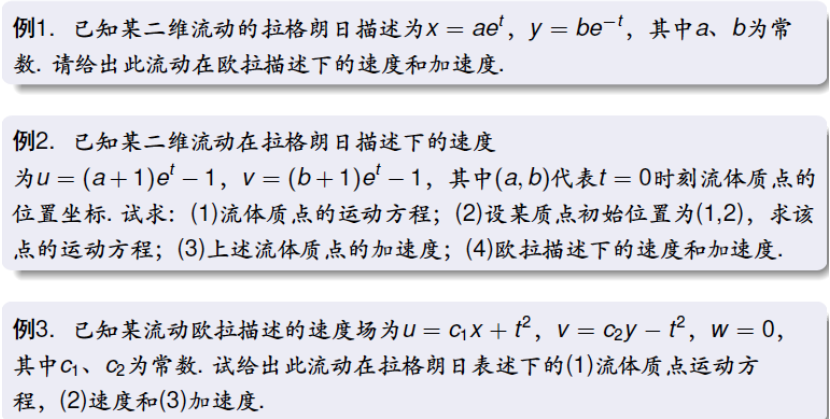
\includegraphics[width=0.9\linewidth]{img/oula2lar.png}
\end{center}

{\color{red} \uline{这个要补题解,先过,同理还有那个可压缩,不可压缩的表达式}}

\subsection{流体运动的几何表示}

\emph{迹线}:同一流体质点不同时刻所在位置的连线。--与拉格朗日描述相关
--同一质点运动规律的几何表示

\emph{流线}:流线上任一点的速度方向与该曲线的切线方向重合,同一时刻不同质点
组成的曲线。--与欧拉描述相联系--是速度场的几何表示

迹线,本身拉格朗日描述就是迹线,如果已知的是x,y,z的描述,能消除参数t就最好了。
因为本身迹线与拉格朗日描述相联系,因此很多时候,求迹线的过程就是欧拉描述转
拉格朗日描述的过程,即:求积分,解ODE。

流线,$\frac{dx}{u} = \frac{dy}{v} = \frac{dz}{w}$,解这个方程就好了。

{\color{cyan} 需要注意的是},对于定常运动,其实只要运动方向定常(本身不是定常运动)的运动,
其流线与迹线是重合的。最好的例子是课本P45的$u = -tx,~~v = t(y+1)$,
可以看出的是如果让u除v,t消除了,这就说明了运动方向不随时间变化,因为$tan \theta = \frac{u}{v}$
!! 而且,在流线(对应欧拉描述),时间t是一个参数(可变的常数),而非变量。
{\color{red} 更多的注意事项需要做题,尤其是错题后补充}

\subsection{流体微团的运动和受力分析}
流体的运动除平动和转动外,还包括变形运动。其中变形包括线变形与角变形。
所以其实可以说流体运动包括平动、转动、线变形、角变形。
线变形指引起流体微元体积大小变化的边长伸缩线变形运动,
角变形是指引起流体微元体积变化的角变形运动。

刚体的速度分解定理:$\vec v = \vec v_0 + \vec \omega \times \vec r =\vec v_0 + \frac{1}{2}(\nabla \times \vec v ) \times \vec r$

线变形速率:线变形运动是指微元各边长发生伸缩的运动,线变形速率定义为\emph{
    单位时间、单位长度的线变形量。
}
如果是二维,那就是平面微元的面积变化率是:$div A = \theta _x + \theta_y$,三维立体微元的
体积变化率是:$div \vec V = \theta_x +\theta_y + \theta_z$,\emph{
    其实就是说:各个方向的线变形速率之和等于面积/体积的变化率(膨胀率/三维是散度)
    ,对了,$\theta_x = \frac{\partial u}{\partial x},
    \theta_y = \frac{\partial v}{\partial y},
    \theta_z = \frac{\partial w}{\partial z}$
}。

\emph{流体速度}的旋度,可以有三个分量($\omega_x,\omega_y,\omega_z$),$\vec \omega = 
\omega_x \vec i + \omega _y \vec j + \omega _k \vec k = \frac{1}{2}rot~\vec v
= \frac{1}{2} \nabla \times \vec v
$,流体速度的的旋度表征了流体本身的自转角速度!

\subsection{亥姆霍兹速度分解定理}

先用泰勒展开,$\vec v = \vec v_0 + \delta \vec v
                    = \vec v_0 + \frac{\partial \vec v}{\partial x} \delta x
                    + \frac{\partial \vec v}{\partial y} \delta y
                    + \frac{\partial \vec v}{\partial z} \delta z
                    = \vec v_0 + [\frac{\partial \vec v}{\partial x},~
                    \frac{\partial \vec v}{\partial y},~
                    \frac{\partial \vec v}{\partial z}] \cdot
                    [\delta x,~\delta y,~\delta z]^T
$,把上式最后一项展开:

%\centering
\begin{center}
$
\begin{bmatrix}

    \frac{\partial u}{\partial x} & \frac{\partial u}{\partial y} & \frac{\partial u}{\partial z} \\
    \frac{\partial v}{\partial x} & \frac{\partial v}{\partial y} & \frac{\partial v}{\partial z} \\
    \frac{\partial w}{\partial x} & \frac{\partial w}{\partial y} & \frac{\partial w}{\partial z}
\end{bmatrix}
\cdot
\begin{bmatrix}
    \delta x \\ \delta y \\ \delta z
\end{bmatrix}
$
\end{center}
把方阵写成对称阵S(变形)和反对称阵A(转动)。
所以本来,$\vec v = \vec v_0 + (S+A)\cdot \vec \delta \vec r$,但是呢?
A是由$\omega$构成的,所以$A \delta \vec r = \frac{1}{2} rot \vec v \cdot \delta \vec r$
。
那么$\vec v = \vec v_0  + \frac{1}{2} rot \vec v +\vec S \cdot \delta \vec r $。
(平动+转动+变形)

\subsection{作用在流体上的力}

\emph{其实上面说的就是:把运动描述清楚了,是运动学,流体相比于原来的
质点(只有平动)、
刚体(平动+转动),
又增加了转动,所以是平动+转动A+变形S
},那现在是时候看看作用在流体上的力了,其实也简单就两类——体积力、表面力。

我觉得:
体积力就是我们之前熟悉的让物体产生平动、转动的来源之重力啊,万有引力,惯性力啥的,
表面力只在面上,比如粘性力,摩擦力,压力啥的,对吧。

跟线变形、角变形类似,这里的质量力也是单位质量受的力,和高数物理学的不一样吧、
表面力也是 得是单位面积受的力;这样描述的好处是啥呢?就是
知道了单位的对吧,那你再乘上总的质量啊,总的面积啊,就物体所受到的
总的力 你就知道了。

{\color{red} 这里不管是质量力还是表面力,PPT里面的表述都很费解啊,一边说力除以体积
/面积 分别是质量力,表面力,一会又说求出来的结果是质量力,表面力在体积、面积上的分布密度。
质量力是质量力的分布密度?不对啊 ,应该是质量力是这个质量所有的质量力的分布密度。同理
表面力是总的表面力的分布密度。}

总之呢,$\vec p_n = lim \frac{\delta \vec p 表面力}{\delta \vec S 面积}$。
然后就把$\vec p_n$叫做应力矢量。$\vec p_n$是某一时刻在M点以n为其法向
的$\delta S$面,在n所指的一侧的流体对于$\delta S$的另一侧流体的作用力。
应力矢量$\vec p_n$的方向,并不与法向n一致,除了有n方向上的分量,还有面上的切向分量。

$\vec p_n = \vec n \cdot \vec P$。
$\vec P$叫做应力张量。
\begin{center}
$
\begin{bmatrix}
    p_nx & p_ny & p_nz
\end{bmatrix}
=
\begin{bmatrix}
    n_x & n_y & n_z
\end{bmatrix}
\cdot
\begin{bmatrix}
    p_{xx} & p_{xy} & p_{xz}\\
    p_{yx} & p_{yy} & p_{yz}\\
    p_{zx} & p_{zy} & p_{zz}
\end{bmatrix}
$
\end{center}

$p_{xx}, p_{yy},p_{zz}$是法向应力分量,其余6个是切向应力分量。

应力张量各个分量的两个下标,
第一个下标表示该应力作用面的法线方向,
第二个下标表示该应力的投影方向。比如$p_{xy}$
表示:作用于外法线方向为x轴正向的面积元上的应力$p_x$
在y轴上的投影分量。

\subsection{本构方程}

广义牛顿粘性定律的假设(斯托克斯假设):
\begin{itemize}
    \item 流体是连续的,它的应力张量是应变率张量的线性函数,与流动的平动、转动无关。
    \item 流体是各向同性,其应力张量与应变率张量之间的关系与坐标系的选择与位置无关。
    \item 当流体静止,应变率为零,流体中的应力就是流体的静压强。
\end{itemize}

$\vec P = 2\mu \vec S + [-p+(\mu' - \frac{2}{3}\mu)\nabla\cdot\vec v]\vec I$
($\mu'$叫第二粘性系数、膨胀粘性系数、度量流体由于体积膨胀或收缩所造成的流体内部能量耗散的系数,一帮
情况下,可以忽略不计,即近似$\mu'=0$)

此即广义牛顿定律,描述了应力张量与应变率张量之间的普遍关系。即牛顿流体的本构方程。

% ====================================================================
\newpage
\section{流体运动基本方程组}

雷诺输运定律就是起到了个,微分转积分的作用?

\begin{description}
    \item[系统] 是指某一确定流体质点集合的总体,即给定流体质点组成的流体团。\emph{相当于原来研究的被简化为质点的物体}
    系统和外界之间有边界隔开;流动过程中,位置和形状可以改变,组成的质点是固定的,
    和外界可以有力的交互作用,动能、能力交换,只是没有物质交换。(是拉格朗日描述)
    \item[控制体] 指流体所在空间中以假想或真实流体边界包围的、固定不动的、形状任意 
    的空间体积,包围控制体的叫控制面。一旦选定,其形状、大小、位置都是确定的,流体呢,不断
    流入流出,是流体的欧拉描述。
    \item[雷诺输运定理] 某时刻一个可变体积的系统上总物理量
    的时间变化率等于该时刻(体积变之前的那个时刻)的空间(控制体)
    中的物理量的时间变化率$+$该流体物理量在单位时间通过该\uline{空间边界}
    净的输运\emph{流体物理量可以是任意矢量物理量}
\end{description}

$\frac{D}{Dt} \int_{\tau(t)} \vec a(\vec r,t)$:
一可变体积系统{\color{red} 总}的物理量(所以对体积积分$\int_{\tau t}$),的时间变化率($\frac{D}{Dt}$)

$\int_{\tau(t)} \frac{\partial \vec a(\vec r,t)}{\partial t}d\tau$
或者说$\frac{\partial}{\partial t} \int_{t}\vec a(\vec r,t) \delta \tau$
:仅仅是时间变化率(所以是对时间的偏微分,$\frac{\partial}{\partial t}$),空间域的所以还是要对空间积分
(备注:$(\vec r,t) = (x,y,z,t)$)

$\oint_{S(t)} \vec a(\vec r,t) \vec v(\vec r,t)\cdot d\vec S$:通过空间域边界(所以对表面积分),单位时间(所以物理量$\times$速度矢量)

散度的物理意义:

三个相互正交方向上线变形速率之和在\emph{向量分析}上称为{\color{cyan} 速度$\vec V$}的散度,
记为$div \vec v$,即
\begin{align*}
    div ~ \vec v = \bigtriangledown \cdot \vec v 
    = \frac{\partial u}{\partial x} + \frac{\partial v}{\partial y}
    + \frac{\partial w}{\partial z}
    = \theta_x +\theta_y + \theta_y
\end{align*}
流体\uline{速度}的散度表示流体微团的相对体积膨胀率(单位时间内单位
体积流体的体积的增长量)
\subsection{连续性方程}
终于到了三大方程!

连续性方程来源是质量守恒定律。可以从系统(拉格朗日)和控制体(欧拉)两种思路来
思考:
1. 包含在一流体系统中的流体质量在流动过程中保持不变;
2. 在一固定空间中的流体质量的减少率等于单位时间内通过其表面的质量通量。

拉格朗日描述下推导连续性方程:
\begin{align*}
    \frac{d}{dt}\delta m &= 0\\
    \frac{d}{dt} (\rho \delta \tau) &= 0\\
    \rho \frac{d}{dt} \delta \tau + \delta \tau \frac{d}{dt} \rho &= 0\\
    \frac{1}{\delta \tau} \frac{d (\delta \tau)}{dt} + \frac{1}{\rho} \frac{d\rho}{dt} &= 0\\
    \because \frac{1}{\delta \tau} \frac{d (\delta \tau)}{dt} &= \nabla \cdot \vec v \\
    \nabla \cdot \vec v +\frac{1}{\rho} \frac{d\rho}{dt} &= 0
\end{align*}
\emph{附:不可压缩:$\rho$不随时间变化,因为如果能压缩
的话,是下一刻发生的。但其在空间分布上可能是不均匀的,所以它是
空间
x,y,z的函数,即$\rho = \rho(x,y,z)$或$div ~\rho = \nabla \cdot \rho = 0$或$\frac{d\rho}{dt}=0${\color{red} 这是有问题的啊。不可压缩对空间不均匀的话,怎么能对时间t求全导数呢?};
均质流体是$\rho = \rho(t)$或$\nabla \rho = 0$;
均质不可压缩:$\rho = const$当然对空间求梯度,对时间求导都是0}

欧拉观点下推导连续性方程:
{\color{red} 我觉得?}:$\oint_S \rho \vec v \cdot d\vec S$是总的流入的增加的;
$-\int_{\tau} \frac{\partial \rho}{\partial t}\delta t$是因为密度变化为减少的。
然后增加的和减少的加起来为零,也就是:
\begin{align*}
    \int_{\tau} \frac{\delta \rho}{\partial t} \delta \tau +
    \oint_S \rho \vec v \cdot d\vec S = 0
\end{align*}
奥-高公式:
\begin{center}
    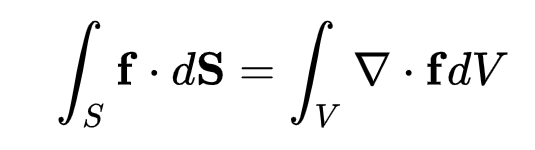
\includegraphics[width=0.4\linewidth]{img/ao-gao.png}
\end{center}
前面的公式可以推导如下:
\begin{align*}
    \int_{\tau} \frac{\delta \rho}{\partial t} \delta \tau +
    \oint_S \rho \vec v \cdot d\vec S &= 0\\
    \int_{\tau} \frac{\delta \rho}{\partial t} \delta \tau + 
    \int_{\tau} \nabla \cdot (\rho \vec v) d\tau &= 0\\
    \int_{\tau} [\frac{\delta \rho}{\partial t} + \nabla \cdot (\rho \vec v) ] \delta \tau &= 0\\
    \therefore \frac{\delta \rho}{\partial t} + \nabla \cdot (\rho \vec v) &= 0
\end{align*}
拉格朗日推导出来的和欧拉推导出来的其实是一样的,
只是暂时长得不一样而已,可以利用标量矢量的积的散度公式互相推导:
\begin{align*}
    div(\varphi \vec F) &= grad(\varphi)\cdot \vec F +\varphi ~ div(\vec F)\\
                        &= (\nabla \varphi)\cdot \vec F + \varphi(\nabla \cdot \vec F)
\end{align*}

雷诺输运定理推导连续性方程:

把雷诺输运定理里面的物理量换成了$\rho$:
\begin{align*}
    \frac{d}{dt} \int_{\tau} \rho d\tau &= 
    \int_{\tau} \frac{\partial \rho}{\partial t} \delta \tau 
    + \oint_S \rho \vec v \cdot d \vec S \\
    \because \frac{d}{dt} \int_{\tau} \rho d\tau &= 0\\
    \therefore \int_{\tau} \frac{\partial \rho}{\partial t} \delta \tau 
    + \oint_S \rho \vec v \cdot d \vec S &= 0\\
    \therefore \int_{\tau} [\frac{\partial \rho}{\partial t} + \nabla \cdot (\rho \vec v)] \delta \tau &= 0\\
    \therefore \frac{\partial \rho}{\partial t} + \nabla \cdot (\rho \vec v) &= 0
\end{align*}
{\color{red} \uline{这些个里面的大S是标量还是矢量,感觉标量也不对,矢量也不太对}}
这里雷诺输运定理右手第一项把偏分写在里面,
没有写外面,
是因为后面正好利用对同一变量的积分
把两个式子加起来!

连续性方程的特殊情况:
\begin{description}
    \item[定常运动] $\frac{\partial \rho}{\partial t} = 0$:$\nabla \cdot (\rho \vec v) = 0$ 单位体积净的流出质量为0(流入流出的质量相等)
    \item[不可压缩流动] $\frac{d\rho}{dt} = 0 \therefore \nabla \cdot \vec v = 0$ ::
     流体微团的体积在其运动过程中保持不变::
     利用奥-高公式$\oint_S \vec v \cdot dS = \int_{\tau} \nabla \cdot \vec v d \tau \therefore$
     对不可压缩,在任意闭合曲面上$\oint_S \vec v \cdot dS = 0$
    \item[均质流体的不可压缩流动] 密度为常数,连续性方程为:$\nabla \cdot \vec v = 0$。
\end{description}
\subsection{运动方程-动量定理}

中学时候,
动量定理的描述一般是$F\delta t = m \delta \vec v$。流体力学里描述是:合外力(质量力加上面力)等于动量的时间变化率。其实就是把$\delta t$给除过去了。

\emph{需要注意的是,质量力或者面积力,分别是单位
质量、单位面积上的力
。}
因此对某一个系统(拉格朗日观点)其体积为$\tau$,边界为S。设质量力为F,面积力为$\vec p_n~~~ \vec p_n = \vec P \cdot \vec n ~~~ \oint _S \vec p_n ds  = \oint _S \vec P \cdot d\vec S $。\emph{也可以理解嘛,应力张量是全的,各个方向的面积力都有,相当于一个字典,我们用的时候索引我们需要的那一部分面积力}。

那对这个系统来说,体积力为$\int _{\tau} \rho \vec F d\tau $,面积力为$\oint _S \vec P \cdot d\vec S ~~or~~ \oint_S \vec p_n ds $,总动量为$\int_{\tau} \rho \vec V d\tau$。

那么,动量定理的关系式子就是:
\begin{align*}
    \frac{d}{dt} \int_{\tau} \rho \vec V d\tau 
     = \int_{\tau} \rho \vec F d\tau 
     + \oint_S \vec p_n ds
\end{align*}

然后(为的是把体积积分,面积积分都换成体积积分,这样不就可以合并到一起了吗),把第一项里的$\rho \vec v d\tau $看做$\vec v(\rho  d\tau)$,把$\frac{d}{dt}$移动到积分号内,
因为$\frac{d}{dt}(\vec v \rho d\tau) = 
\vec v  \frac{d}{dt} \rho d\tau 
+ \rho d\tau \frac{d}{dt} \vec v
$,因为质量守恒($\frac{d}{dt} \rho d\tau = 
\frac{d}{dt} dm = 0$),所以$\frac{d}{dt} \int_{\tau} \rho \vec V d\tau = \int_{\tau} \frac{d\vec v}{dt}
\rho d\tau$
;
把第三项的$\oint_S \vec p_n ds$看做
$\oint_S \vec P \cdot d\vec s$,加上奥高公式,变成了
$\int_{\tau} \nabla \cdot \vec P d\tau$。

那么,动量定理的式子就变成了:
\begin{align*}
    \int_{\tau} \frac{d\vec v}{dt} \rho d\tau
        &= \int_{\tau} \rho \vec F d\tau
        + \int_{\tau} \nabla \cdot \vec P d\tau\\
    \rho \frac{d\vec v}{dt} &= \rho \vec F +
    \nabla \cdot \vec P
\end{align*}

加上利用本构方程:$\vec P = 
2\mu \vec S -
[p + \frac{2}{3}\mu \nabla\cdot \vec v] \vec I
$
,连续性方程就变成了:

\begin{align*}
\rho \frac{d\vec v}{dt} 
    = \rho \vec F
    - \nabla p 
    + \nabla \cdot (2\mu \vec S)
    - \frac{2}{3} \nabla (\mu \nabla \cdot \vec v)
\end{align*}

这就是Navier-Stokes方程,

\begin{description}
    \item[左端] 单位体积流体的惯性力
    \item[右端第一项] 单位体积流体受到的质量力
    \item[右端第二项] 单位体积流体的压强梯度力
    \item[右端第三项] 粘性变形应力
    \item[右端第四项] 粘性体积膨胀应力
\end{description}

对于不可压缩流动,因为$\nabla \cdot \vec V = 0$,
且若$\mu$为常数,那么可以简化为:

\begin{align*}
\rho \frac{d\vec v}{dt}
 = \rho \vec F
 - \nabla p
 + \mu \nabla ^2 \vec v
\end{align*}

\begin{description}
    \item[理想流体] 因$\mu=0,P = -p\vec I$,方程简化为:$\rho \frac{d\vec v}{dt}
 = \rho \vec F
 - \nabla p$。欧拉方程
    \item[流体静止不动] $\vec v=0$:方程简化为:$ \rho \vec F = \nabla p $.静力学方程 
    \item[兰姆-葛兰米柯方程] 将位变加速度分为位势部分和涡旋部分$(\vec v \cdot \nabla )\vec v = \nabla \frac{{\vec v} ^2}{2} + (\nabla \times \vec v)\times \vec v$,方程变化为:
    $\rho(\frac{\partial \vec v }{\partial t}
    + \nabla \frac{{\vec v} ^2}{2} + (\nabla \times \vec v)\times \vec v) 
    = \rho \vec F
 - \nabla p$。
\end{description}

\subsection{能量方程}

能量方程是热力学第一定律的具体表现,(热力学第一定律:$\Delta E_{nei'neng} = Q(chuan're)+W(zuo'gong)$)。

对单位质量的流体的内能是$e$,动能是$k$,则体积$\tau$内的总能量是:$E(t) = \int_{\tau} \rho (e+k) d\tau$

质量力和面力做的功分别是:$\int _{\tau} \rho \vec F \cdot \vec v d \tau $,和$\oint _S \vec p_n \cdot \vec v ds$

传热包含两种情况,热传导和辐射。单位时间由于热传导通过S进入$\tau$的热量是$\oint _S k \nabla T \cdot d\vec s = \oint_S k \frac{\partial T}{\partial n} ds$。
单位时间内由于热辐射传入单位质量流体的质量为$q$,那么单位时间由于辐射进入$\tau$的热量为$\int_{\tau} \rho q d \tau$。

因此,由热力学第一定律有:
\begin{align*}
    \frac{d}{dt} \int_{\tau} \rho (e+k) d\tau
      = \int _{\tau} \rho \vec F \cdot \vec v d \tau
      + \oint _S \vec p_n \cdot \vec v ds
      + \oint _S k \nabla T \cdot d\vec s
      + \int_{\tau} \rho q d \tau
\end{align*}
为了得到一个能量方程,肯定得合并,需要做两个事情——微分变积分,面积分变体积分。

上面这个方程呢,左边第一项是一个微分的形式想要变成积分,有两种方法——一个是使用随体导数加上质量守恒,一个是雷诺输运定理。

\begin{center}
    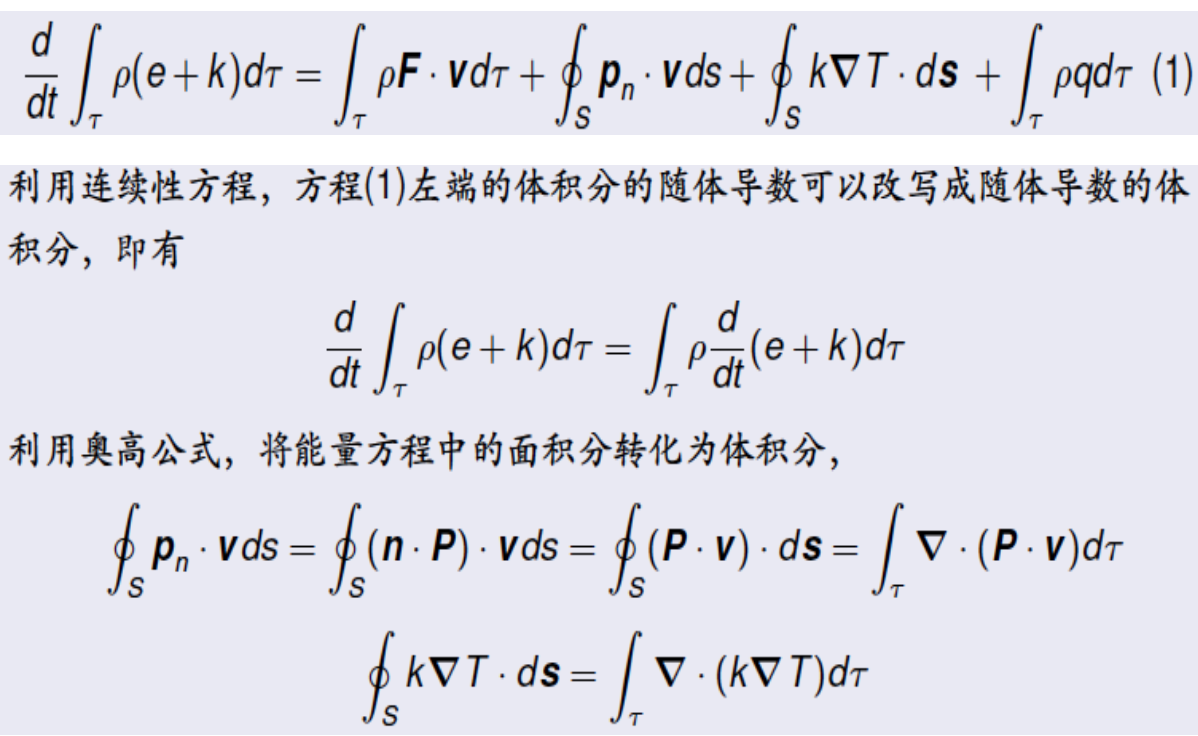
\includegraphics[width=0.8\linewidth]{img/energy1.png}
    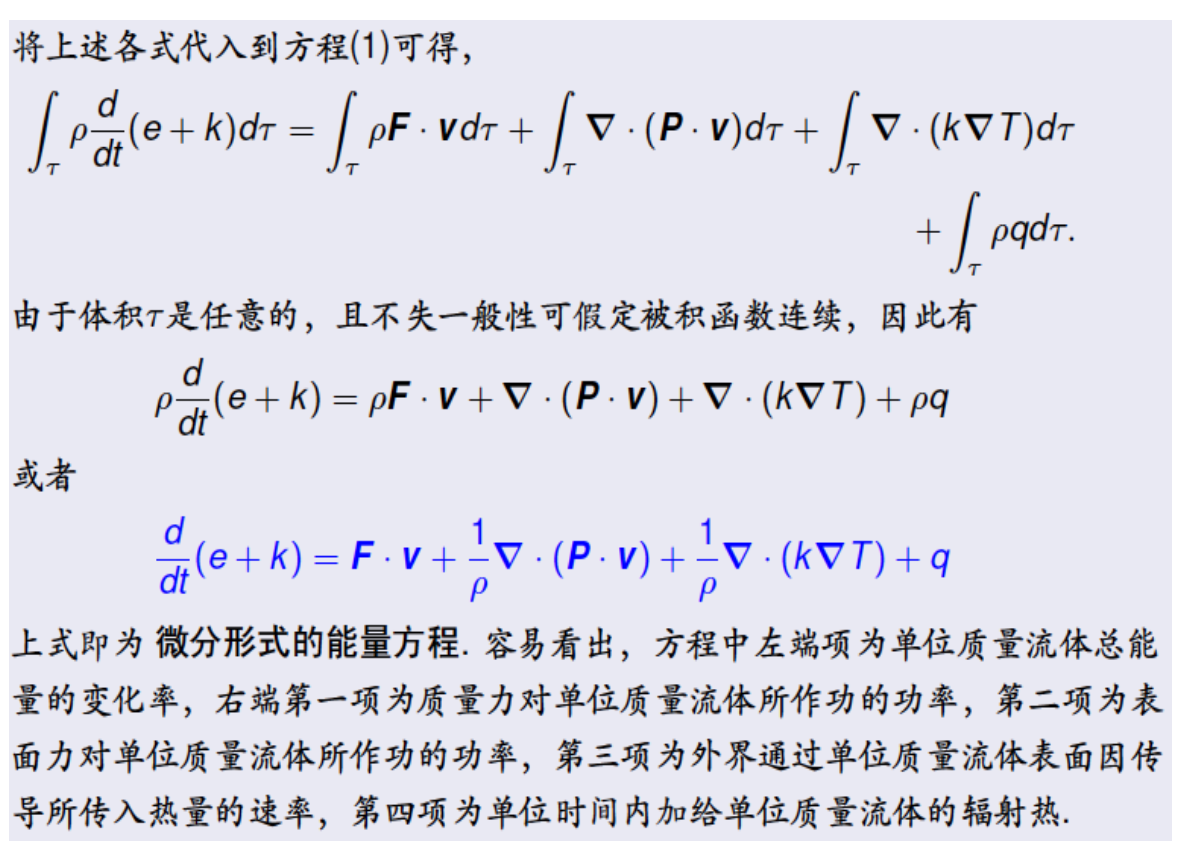
\includegraphics[width=0.8\linewidth]{img/energy2.png}
\end{center}

\subsection{动能方程}
这部分先跳过直接复制粘贴PPT吧。

\subsection{状态方程}

对于均值的平衡态,描述其热力学状态的独立变量只有两个,压强P和温度T,其余的状态变量都可以表示成压强P和温度T的函数,这个函数就称为状态方程。比如:
\begin{description}
    \item[理想气体] 经典的$PV= nRT$
    \item[海水] $\rho = \rho(p,T,S)$
\end{description}

\subsection{定解条件}

想确定具体的流动(找出流体力学方程组的确定的解),必须给出方程组的定解条件,包含:初始条件($t=0$时的状态)和边界条件。

\[
\begin{cases}
  \vec v(\vec r,t_0) = \vec v_0(\vec r) \\ 
  \rho(\vec r,t_0) = \rho_0(\vec r) \\ 
  p(\vec r,t_0)  = p_0(\vec r) \\ 
  T(\vec r,t_0) = T_0(\vec r)
\end{cases}
\]

边界条件:
\begin{itemize}
    \item 物质面两侧质点速度一致
    \item 热通量密度相等
    \item 对粘性介质,无滑移边界条件
\end{itemize} 

\section{涡旋运动}

涡量:速度的旋度$\omega = \nabla \times \vec v$等于角速度的两倍。
涡量各点构成一个矢量场,称为涡量场。

涡旋:一群绕公共质心旋转的流体微团,或,以无旋流体或物面
为边界的有限体积的有旋流体。

某时刻的涡管,取涡管的一个横截面A,过曲面A的涡通量
为该瞬时的涡管强度。

涡通量:某一曲面积分$I = \int_s \omega \cdot d\vec s$
(被积函数是速度的偏导数)

速度环量:某时刻封闭曲线L,$\varGamma = \oint_L \vec v \cdot \vec l$
(积分函数是速度本身)

涡管强度守恒定律:
\begin{description}
    \item[1] 同一时刻同一涡管,涡通量是相同的,涡管强度守恒,与截面选取无关。
    \item[2] 面积越小,涡量越大,流体旋转角速度越大。
    \item[3] 涡管截面不可能收缩为零,因此涡管不能在流体之中产生或终止
\end{description}

粘性流体的\emph{涡量输运方程}:
\begin{align*}
    \frac{d\boldsymbol \omega}{dt} 
        = (\boldsymbol \omega \cdot \nabla) \boldsymbol v
        - \boldsymbol \omega(\nabla \cdot \boldsymbol v)
        + \nabla \times \boldsymbol F
        + \frac{1}{\rho^2}\nabla\rho \times \nabla p
        + \nu \nabla ^2 \boldsymbol \omega
\end{align*}

各项物理意义(影响涡量变化的各种物理机制):
\begin{enumerate}
    \item $(\boldsymbol \omega \cdot \nabla) \boldsymbol v$ 表示速度沿着涡线的变化,分解成两部分,垂直或水平。
    表征了
    由于流场空间分布不均匀,涡线将发生拉伸和扭曲,
    导致涡量场的变化。
    \item $\boldsymbol \omega(\nabla \cdot \boldsymbol v)$散度项,表示流体微团的体积变化引起的涡量大小发生的变化(体积变化,比如增大时,转动惯量增加,转动角速度减小,涡量减小。)
    \item $\nabla \times \boldsymbol F$ 体积力的贡献,如果体积力有势,如$F = -\nabla \phi$该项为零,表征了 非保守力对涡量的贡献。
    \item $\frac{1}{\rho^2}\nabla\rho \times \nabla p$ 该项不等于零表示热力学里面有两个独立变量,具有这种性质的流体称作斜压流体,反之只有一个独立变量的流体称为正压流体。这项表示流体的斜压性,使得等密面和等压面斜交$\nabla\rho \times \nabla p$,使得涡量发生变化
    \item $\nu \nabla ^2 \boldsymbol \omega$ 粘性扩散项,表示涡量的粘性扩散效应
\end{enumerate}

刚刚上面这个解释了影响涡量大小变化的因素,下面是影响速度环量$/$涡通量$/$涡管强度的几个因素。
推导思路是:上面说了速度环量比较常用,因为积分对象是速度本身,我们就选择对速度环量进行求随体导数。

结果表明:\uline{体积力、流体斜压性和粘性}是引起速度环量、涡通量变化的三个因素。

亥姆霍兹方程:

假设流体是理想流体(粘性系数$\nu = 0$),体力有势,流体是正压的,
则涡量输运方程可以简化为:
\begin{align*}
        \frac{d\boldsymbol \omega}{dt} 
        = (\boldsymbol \omega \cdot \nabla) \boldsymbol v
        - \boldsymbol \omega(\nabla \cdot \boldsymbol v)
\end{align*}

即 亥姆霍兹方程,无粘正压流体在保守力作用下的涡量输运方程。

开尔文定理:

对于体力单值有势的正压流体的无粘流动,沿着任意可收缩物质周线上的速度环量是个运动不变量。

{\color{red} 就算没上述假设,速度环量不也是不变的吗 因为 速度环量就是涡管强度,之前有涡管强度保持性定理}

亥姆霍兹第一定理:

若流体理想,正压,且外力有势,则在某时刻组成涡线、涡面或者涡管的流体质点在以前或者以后任一时刻也永远组成涡线,涡面,或者涡管。

亥姆霍兹第二定理:

若流体理想,正压,且外力有势,则涡管的强度在运动过程中恒不变。

\subsection{涡旋引起的速度场}

已知流体的涡量和散度,怎样确定流体的速度?

基本思路是:把速度分解成一个有势v1一个有旋v2两部分之和。(有势的求旋度为零,有旋的求散度为零)。

\subsection{直线涡丝感生的速度场}

比奥萨瓦尔公式:
\begin{align*}
    \boldsymbol v &= \frac{\Gamma}{4\pi} \int_L \frac{d\boldsymbol I\times \boldsymbol R}{R^3}\\
    &= \frac{\Gamma}{4\pi} \int_{\alpha_1}^{\alpha_2} 
          \frac{sin\alpha}{h}d\alpha\boldsymbol e_\theta \\
        &= \frac{\Gamma}{4\pi h}(cos\alpha _2  - cos\alpha_1)\boldsymbol e_\theta
\end{align*}

如:该涡丝是无限长的,那么$\alpha _2 = 0, \alpha_1 = \pi$。
那么其感生出来的速度场:
\begin{align*}
    \boldsymbol v = \frac{\Gamma}{2\pi h} \boldsymbol e_\theta
\end{align*}

速度场的特点是:
\begin{enumerate}
    \item 速度方向沿圆周切线方向,该圆周在与直线涡丝垂直的平面内,且以直线涡丝与平面的交点为圆心。
    \item 速度大小除以涡线强度$\Gamma$有关外,只与所有点到直线涡丝的垂直距离h有关。
\end{enumerate}

\subsection{涡旋运动的产生、扩散和衰减}

速度环量的不守恒性来源于:非保守力、斜压性和粘性。

在旋转系统(地球流体系统)中,除了斜压性和粘性外,科氏力也可以导致涡线的生成或衰减。

只有斜压作用的情况下:斜压性会使速度环量发生变化。

无限大平板突然启动,匀速U。
\emph{主要思路是:有三大方程\&涡量方程,我们只写出运动方程和涡量方程。然后建立坐标系,
找出哪几个速度一直是0,然后简化方程;设初始条件+边界条件;然后解方程ODE。
}

这些题目都是涡量沿着壁面传播扩散的,壁面首先需要有粘性,壁面还得存在压强梯度,这是壁面涡量进入流体的必要条件。两个例子,一个无限长直涡线,一个是无限大平板。

虽然但是,{\color{red} 还是不太懂运动方程里把体积力去掉的原因。}

\begin{figure}[h]
    \centering
    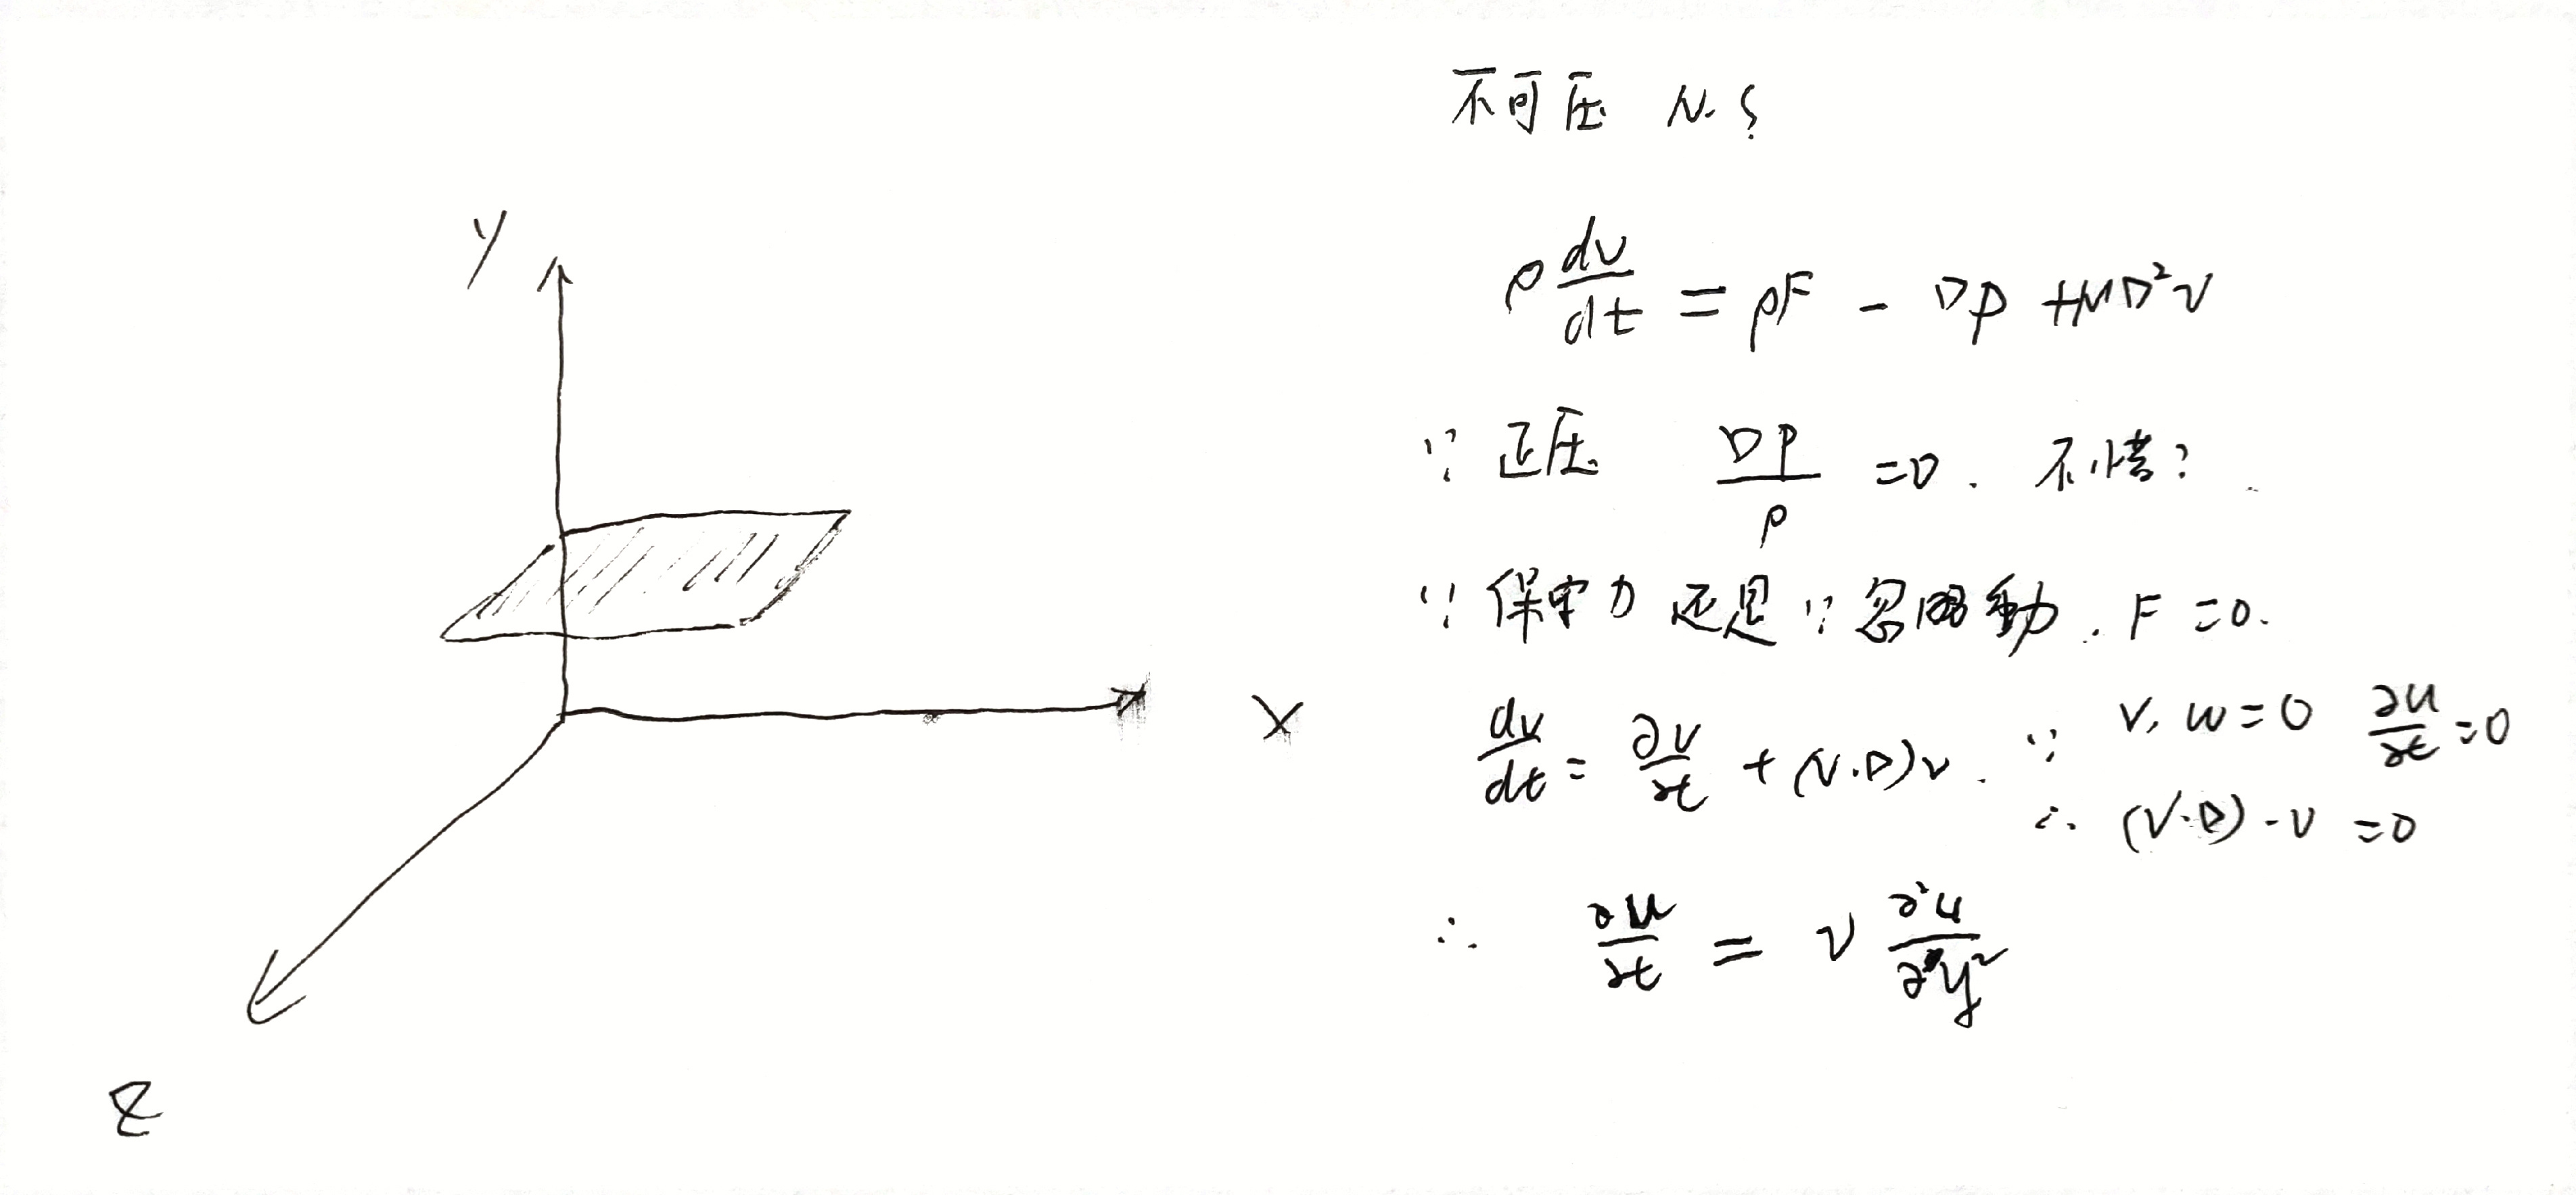
\includegraphics[width=0.8\linewidth]{img/IMG_20201226_1102251.jpg}
   % \caption{示意图}
%    \label{fig:my_label}
\end{figure}

定解条件,$t=0$时,$u=0$;$t>0$时,在$y=0$处,$u=U_0$,在$y\rightarrow \infty$处,$u=0$.

引入无量纲自变量$\eta = \frac{y}{2\sqrt{\nu t} },~ u_{\star} = \frac{u}{U_0} = f(\eta ) $

  动力学方程则变化为:
  \begin{align*}
    f^{\prime \prime }  + 2\eta f^{\prime } = 0
  \end{align*}
  
  定解条件为:$f(0) = 1,~ f(\infty) = 0$ 

  上述微分方程的解为:
  \begin{align*}
    \frac{u}{U_0} = u_{\star} = 1 - \frac{2}{\sqrt{\pi}} \int_0^{\eta} e^{-\eta^2}d\eta
  \end{align*}
  
  那么,$u = U_0 u_{\star} = U_0 - \frac{2U_0}{\sqrt{\pi}} \int_0^{\eta} e^{-\eta^2}d\eta$

$\omega = -\frac{\partial u}{\partial y} = \frac{U_0}{\sqrt{\pi \nu t}}e^{-\frac{y^2}{4\nu t}}$

\section{无粘流体运动学基础}

\subsection{流体运动的相似性理论}

实验模拟怎样才和真实流动有对应关系?——相似性理论

物理量与其特征量之比,称为无量纲物理量。
特征物理量:相似流动中某一指定状态的物理量。
(相似流动中只需要一个无量纲解,就可以通过无量纲关系得到位似系统中任意流动的解)

相似流动的充要条件是:几何相似的牛顿型流体的流场中,无量纲数相等,则流动相似。

\begin{description}
    \item[雷诺数] $Re = \frac{\rho UL}{\mu} = \frac{UL}{\nu}$ Re是相似流场中惯性力和粘性力量级之比({\color{red} 量级之比是什么意思}) 
    \item[弗劳德数] $Fr = \frac{\frac{U^2}{L}}{g}$ Fr是相似流场中惯性力和重力量级之比(所以重力有重要作用的流场Fr是关键的无量纲数)
    \item[施特劳哈尔数St] $St = \frac{\frac{U}{T}}{\frac{U^2}{L}} = \frac{L}{UT}$ St是相似流场中局地加速度和对流加速度量级之比,所以St是流动非定常性的标志,对于定常流动,没有特征时间,所以不需要St相似。 
    \item[欧拉数Eu] Eu是压强梯度力和惯性力量级之比,We是表面张力和压强间量级之比 
    \item[马赫数Ma] $Ma = \frac{U}{c}$流速与声速量级之比
    \item[罗斯贝数Ro] $Ro = \frac{U}{\Omega L}$ 惯性力和克氏力量级之比 
\end{description}



\subsection{无粘流动的基本方程组}

\begin{center}
    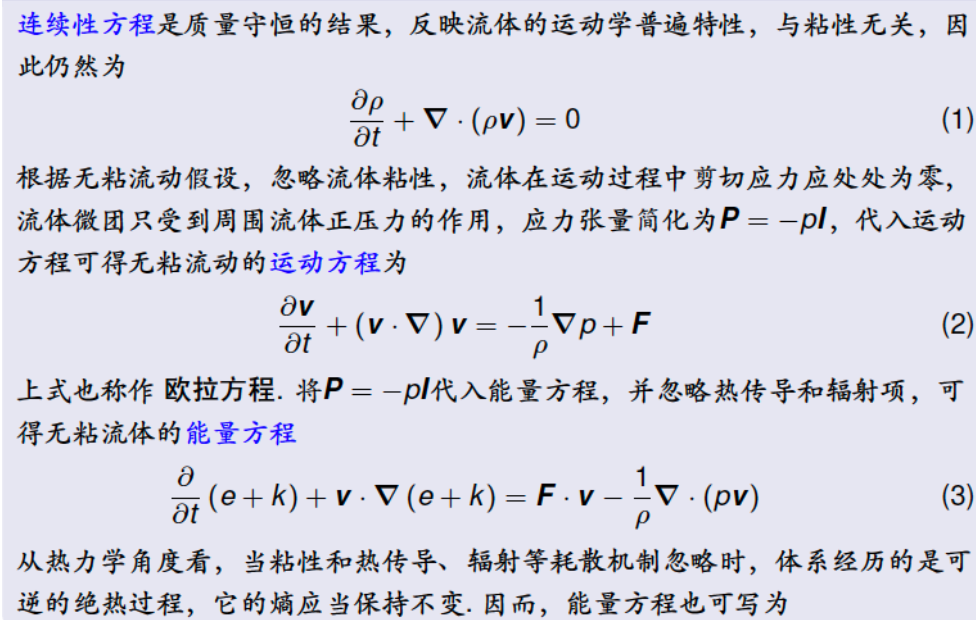
\includegraphics[width=0.8\linewidth]{img/equation1.png}
    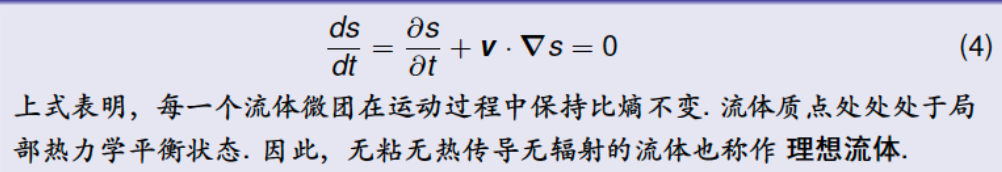
\includegraphics[width=0.8\linewidth]{img/equation2.png}
\end{center}

\subsection{伯努利积分和拉格朗日积分}

伯努利积分就是把上面的运动方程,在假设{\color{red} 流体正压、体力有势、定常、沿着流线 }的情况下,点乘$\boldsymbol s = \frac{v}{V}$就得到了。然后这个$P, \varpi$在可压缩、不可压缩、有旋、无旋的定常流下分别给出
$P, \varpi$的结果,代入就得到了具体情况下的伯努利积分。

比如:伯努利积分为:
\begin{align*}
    \frac{V^2}{2} + P + \Pi = C(\psi)
\end{align*}

对于不可压缩流动:$ d(\frac{p}{\rho}) = \frac{dp}{\rho},~ P = \int \frac{dp}{\rho} = \frac{p}{\rho}$,假设体积力仅仅为重力,即$\Pi = gz + const$
,那么伯努利积分就变成了:
\begin{align*}
    \frac{V^2}{2} + \frac{p}{\rho} + gz = C_1(\psi)
\end{align*}

推导过程:PPT

物理意义:能量守恒的数学表达,左边三项分别是单位质量流体的:动能、压力能和重力势能。
伯努利积分表明了,单位质量流体的总能量沿着流线保持不变。$C(\varphi)$
物理意义是不同流线上单位质量流体的总能量,由于定常流动中流线与迹线重合,伯努利积分也表示\uline{流体质点}在运动过程中总能量守恒。

拉格朗日积分,把上面的运动方程,无粘正压体力有势(\emph{没有定常这个条件}),加上了无旋这个条件,因为$\nabla \times \boldsymbol v = 0$,所以存在速度势,使得$\boldsymbol v = \nabla \varphi$。代入后得到了(倒也不是很复杂)。

拉格朗日积分:
\begin{align*}
    \frac{\partial \varphi}{\partial t} + \frac{V^2}{2} + P + \Pi  = f(t)
\end{align*}

注意,这个f(t)是会随时间变化的常数,但是对一固定时刻t,f(t)在整个流场中是同一个常数,且适用于流场中任何点。

\emph{如果把拉格朗日积分啊,加上不可压缩,体积力为重力的条件},上式变为:$\frac{\partial \varphi}{\partial t} + \frac{p}{\rho} + gz = f(t)$,如果再加上既是物旋又是定常的,那么$\frac{\partial \varphi}{\partial t} = 0, f(t) = const$,于是拉格朗日积分变为:
\begin{align*}
    \frac{\partial \varphi}{\partial t} + \frac{p}{\rho} + gz = C
\end{align*}

\emph{称为伯努利-拉格朗日积分,}这个积分既有伯努利的性质-表达式,又有拉格朗日积分的影子-流场内任意一点在某个时刻值都相等。不同的是,不仅仅是沿着流线、或时刻固定,他任意时刻任意点均是同一个值。

\subsection{速度势和流函数}

无旋必有势,即$\nabla \times \boldsymbol v = 0 \Longleftrightarrow \boldsymbol v = \nabla \varphi$ 称$\varphi$为速度势。带入\uline{不可压缩}的连续性方程,$\nabla ^2 \varphi = 0$,已知速度势和速度后,代入拉格朗日方程,对于\uline{有势体力、无粘、不可压缩、正压、无旋}可以就很容易算出压强p。

对于平面不可压缩流动,连续性方程是$\nabla \cdot \boldsymbol v = \frac{\partial u}{\partial x}+\frac{\partial v}{\partial y} = 0$,引入一个标量函数$\psi$,
使得$\boldsymbol v = \nabla \times  (0,0,\psi) = \frac{\partial \psi}{\partial y} \boldsymbol i - \frac{\partial \psi}{\partial x} \boldsymbol j$

即

\begin{align*}
    u = \frac{\partial \psi}{\partial y}, ~~ v = -\frac{\partial \psi}{\partial x}
\end{align*}

$\psi$这个标量函数称为流函数,流函数具有如下性质:

 \begin{enumerate}
    \item 等流函数线是流线
    \item 平面内任意两点流函数值的差等于通过这两点连线的流量
    \item 流函数$\psi $的值是速度的矢量势的模。
  \end{enumerate}

根据势函数、流函数定义,在平面直角坐标系里面{\color{red} 重要、计算题}:

\begin{align*}
    u &= \frac{\partial \varphi}{\partial x} = \frac{\partial \psi}{\partial y}\\
    v &= \frac{\partial \varphi}{\partial y} = - \frac{\partial \psi}{\partial x}
\end{align*}

\section{粘性流体运动学基础}

\subsection{粘性不可压缩流动的基本方程组}

\begin{figure}[h]
    \centering
    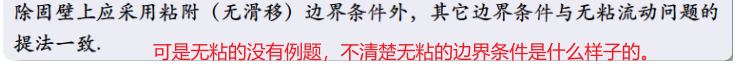
\includegraphics[width=.8\linewidth]{img/wunian-bianjie-ques.png}
    %\caption{Caption}
    %\label{fig:my_label}
\end{figure}

其实最经典的NS方程就是:

\begin{align*}
    \frac{d \boldsymbol v}{dt} = \boldsymbol F - \frac{1}{\rho} \nabla p + \nu \nabla ^2 \boldsymbol v
\end{align*}

当然也可以拆解成三个坐标分量的形式。

\subsection{粘性流动的一般性质}

\subsection{粘性不可压缩流动的解析解}

\begin{figure}[h]
    \centering
    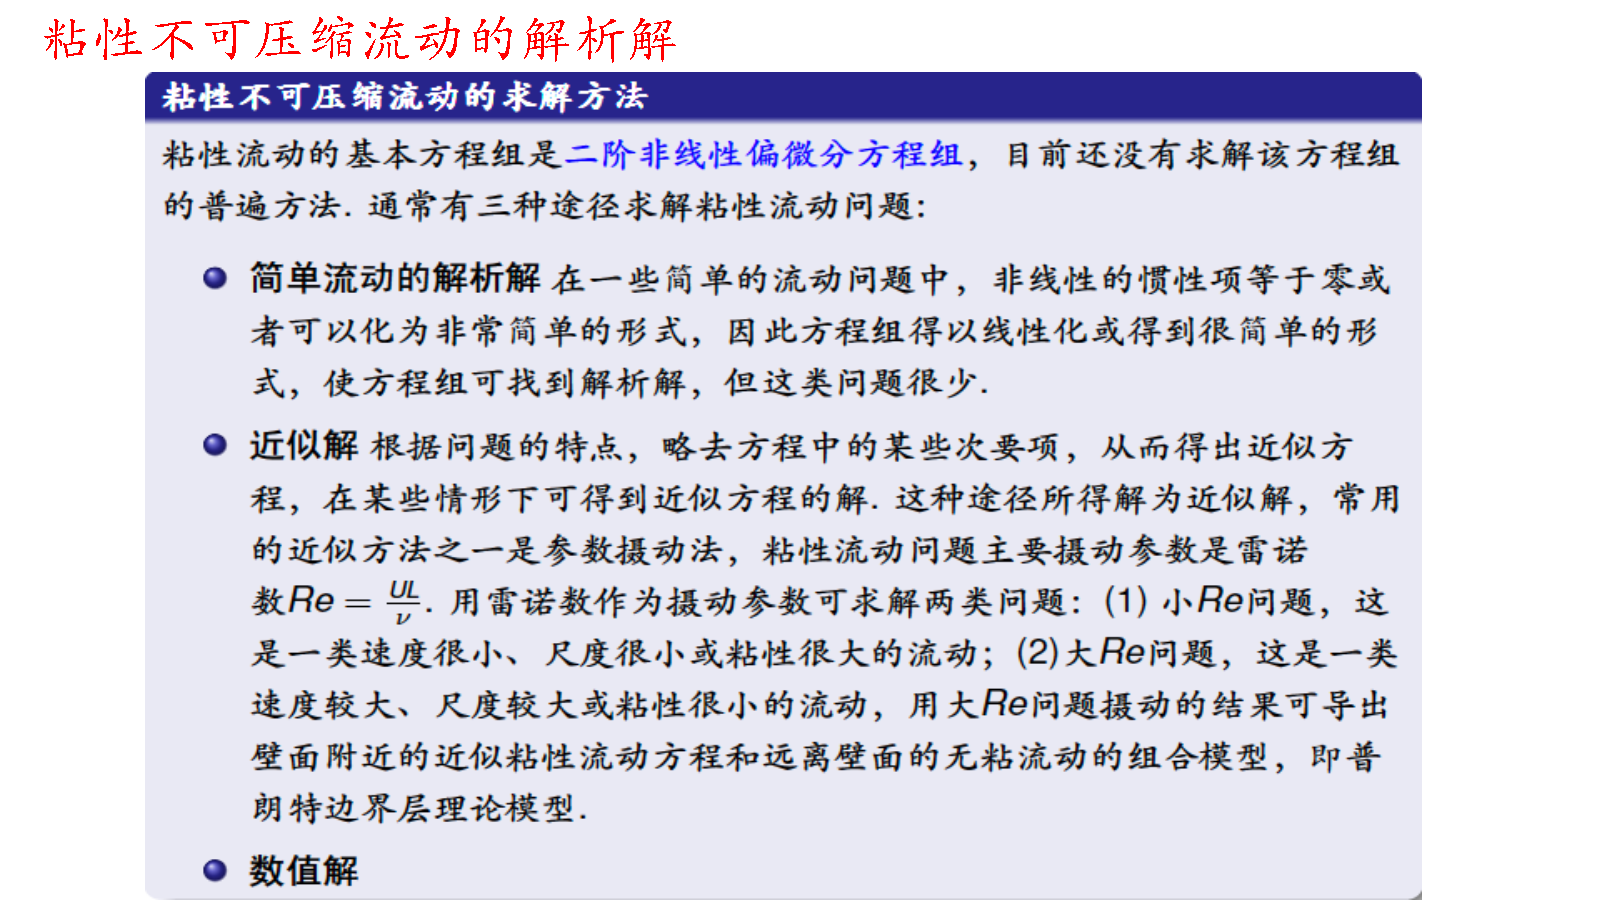
\includegraphics[width=.8\linewidth]{img/cal-2018_06_Page1.png}
    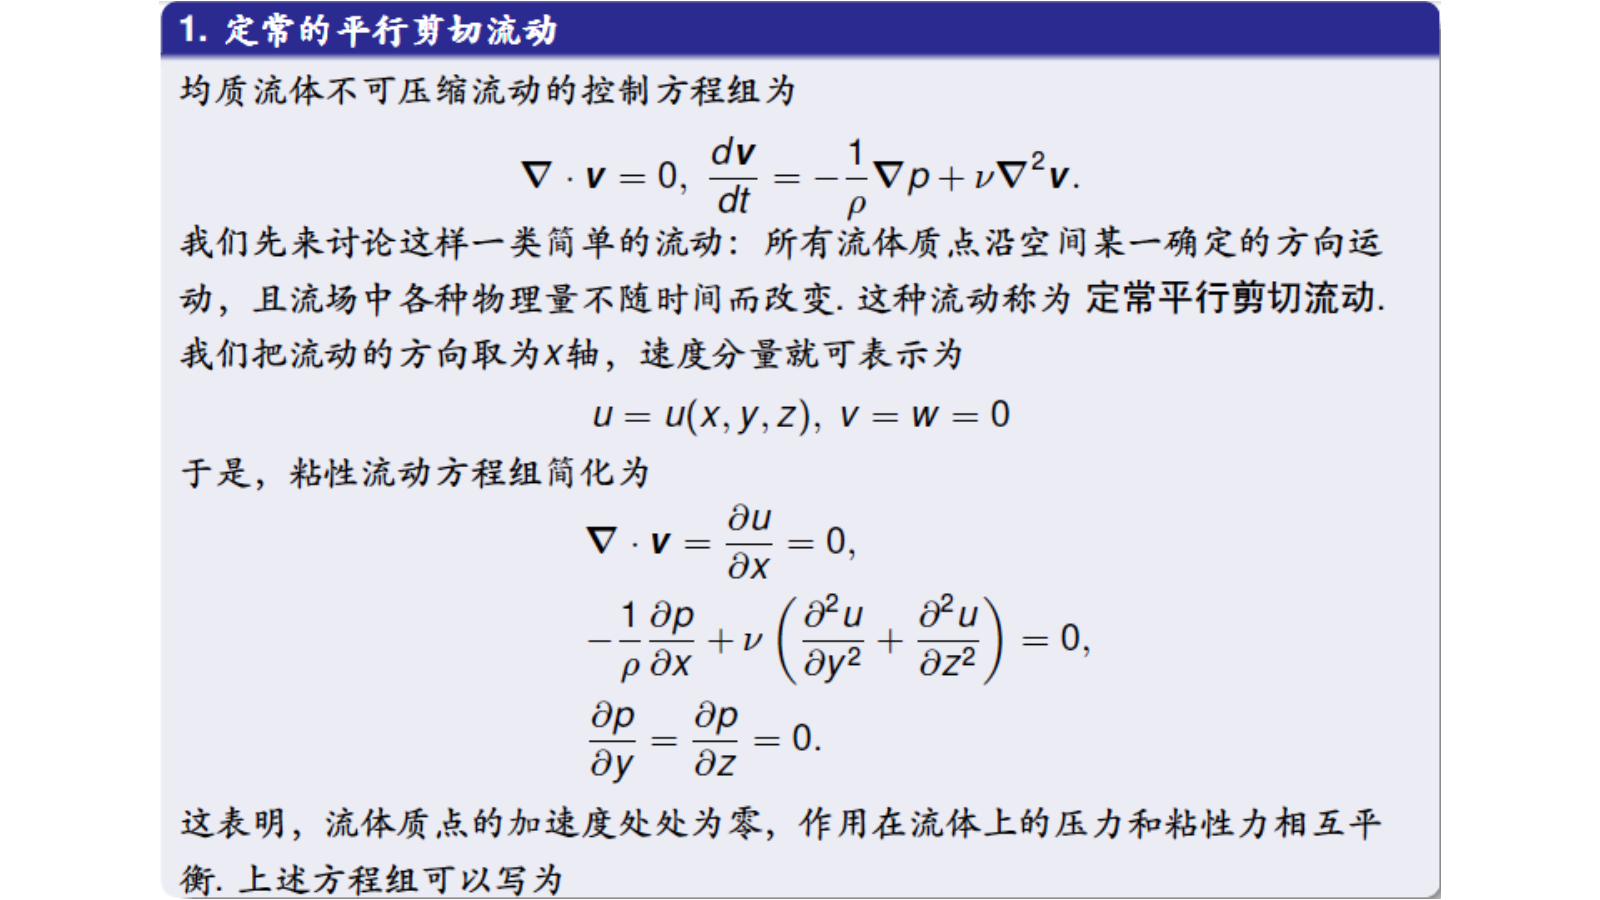
\includegraphics[width=.8\linewidth]{img/cal-2018_06_Page2.png}
    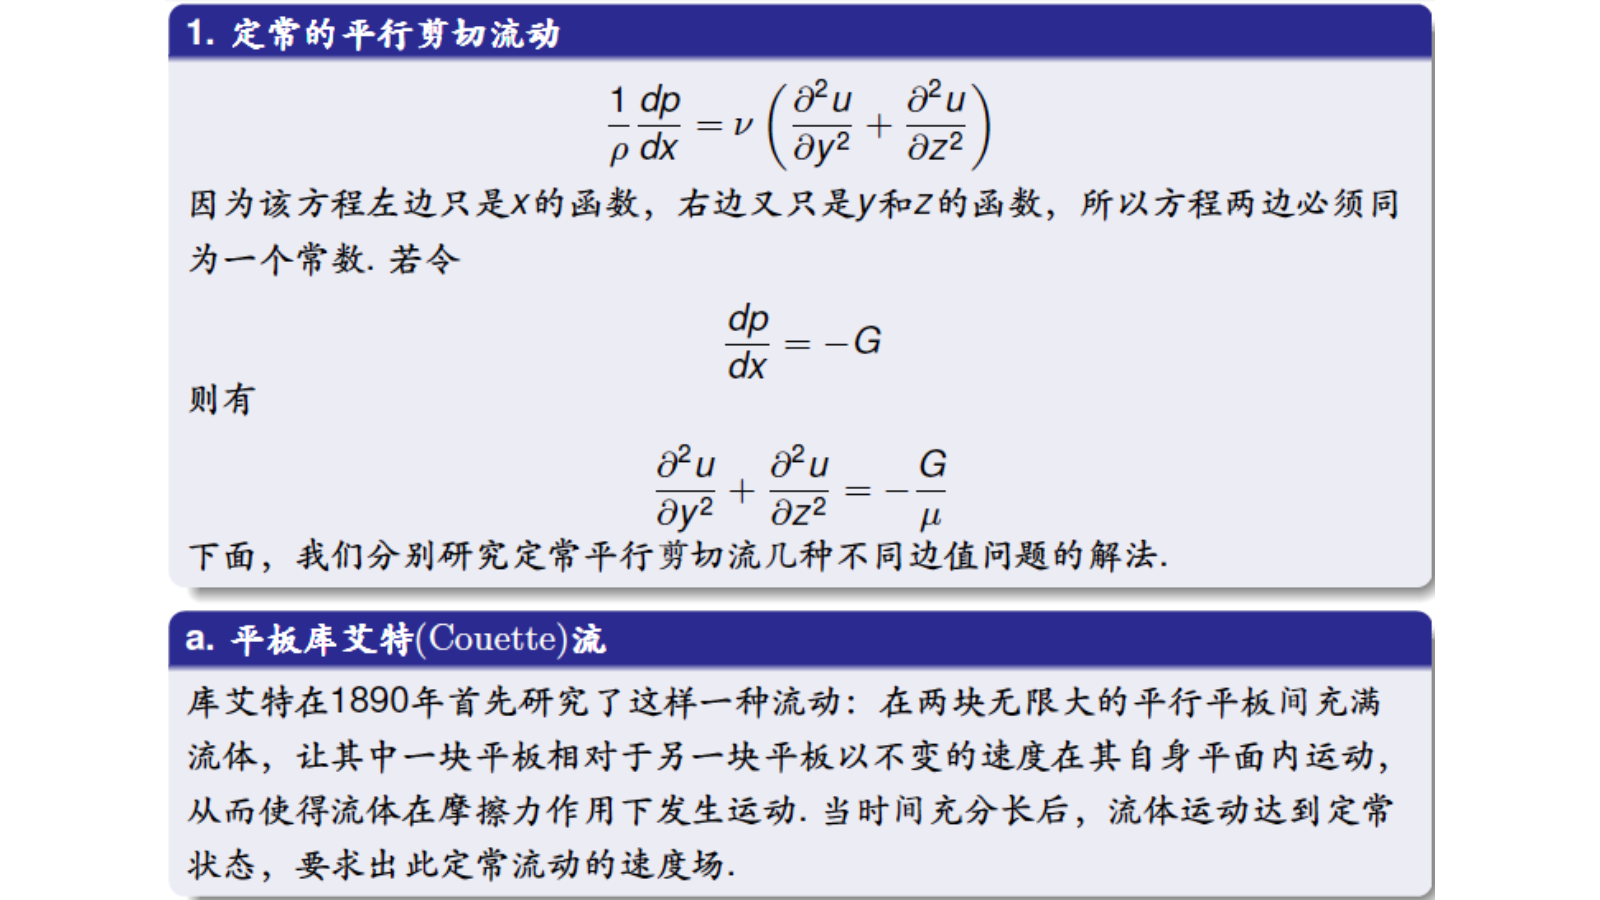
\includegraphics[width=.8\linewidth]{img/cal-2018_06_Page3.png}

\end{figure}

\begin{figure}[h]
    \centering
    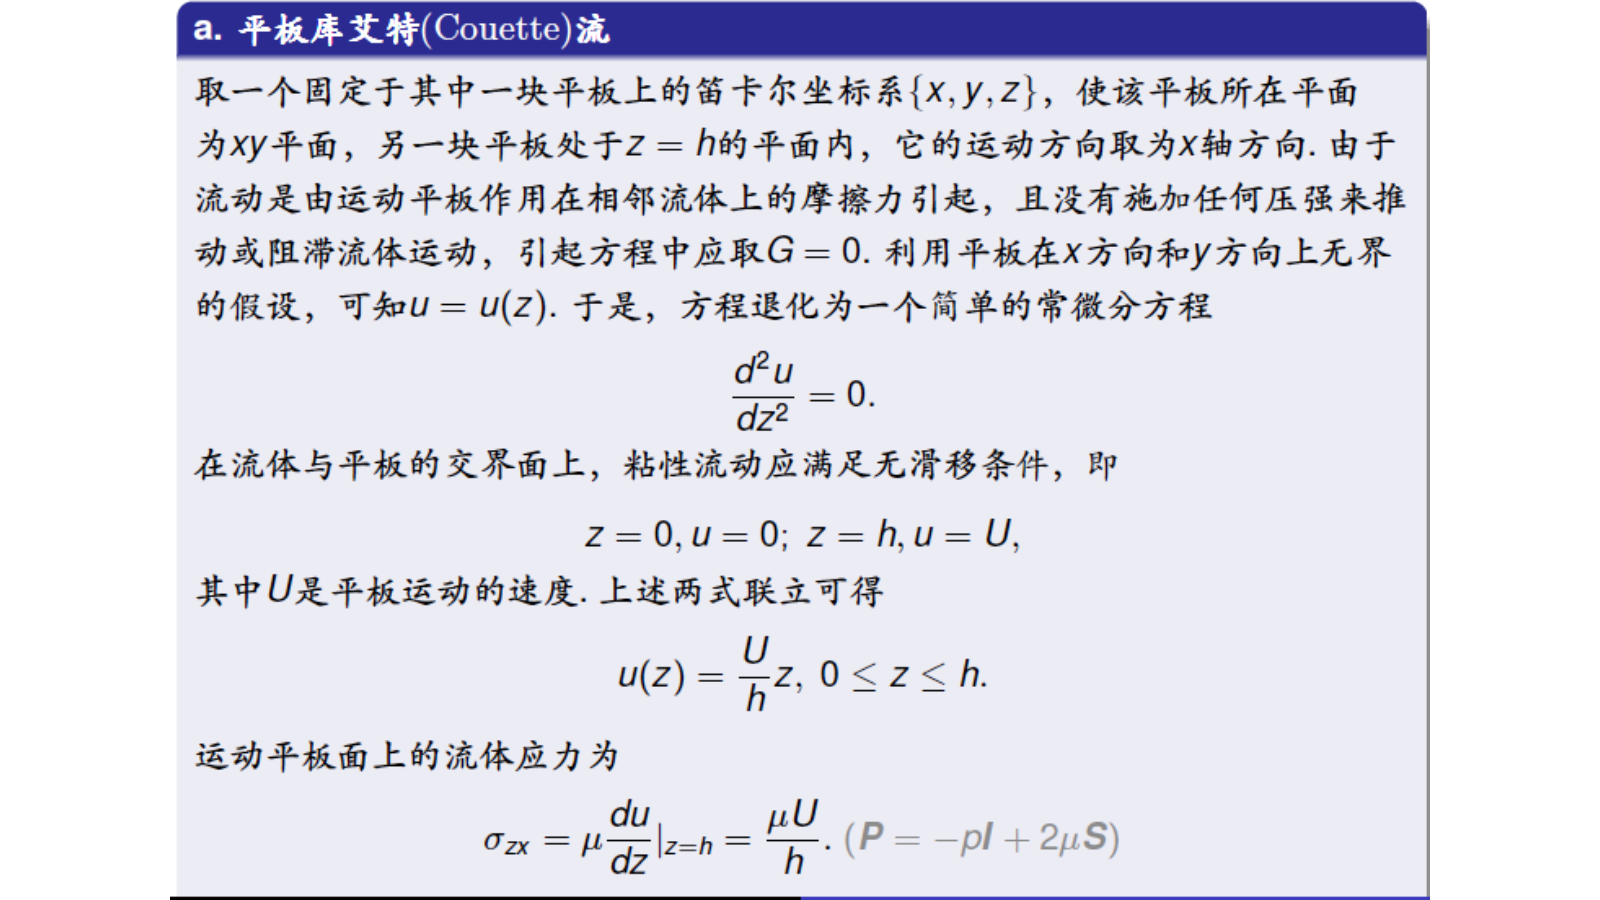
\includegraphics[width=.8\linewidth]{img/cal-2018_06_Page4.png}
    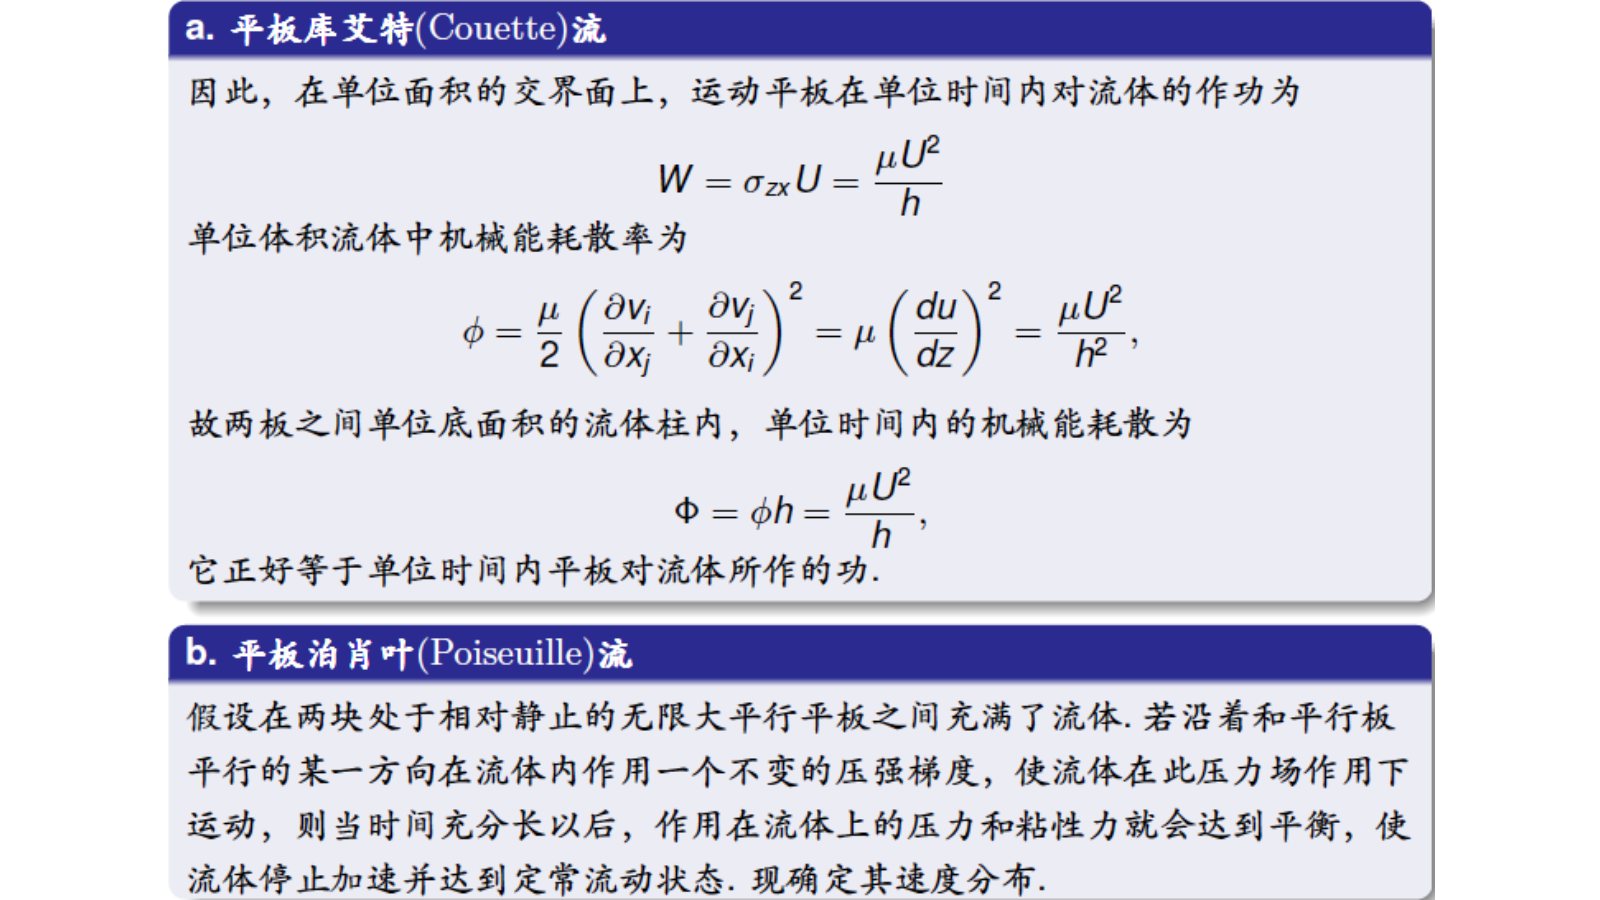
\includegraphics[width=.8\linewidth]{img/cal-2018_06_Page5.png}
    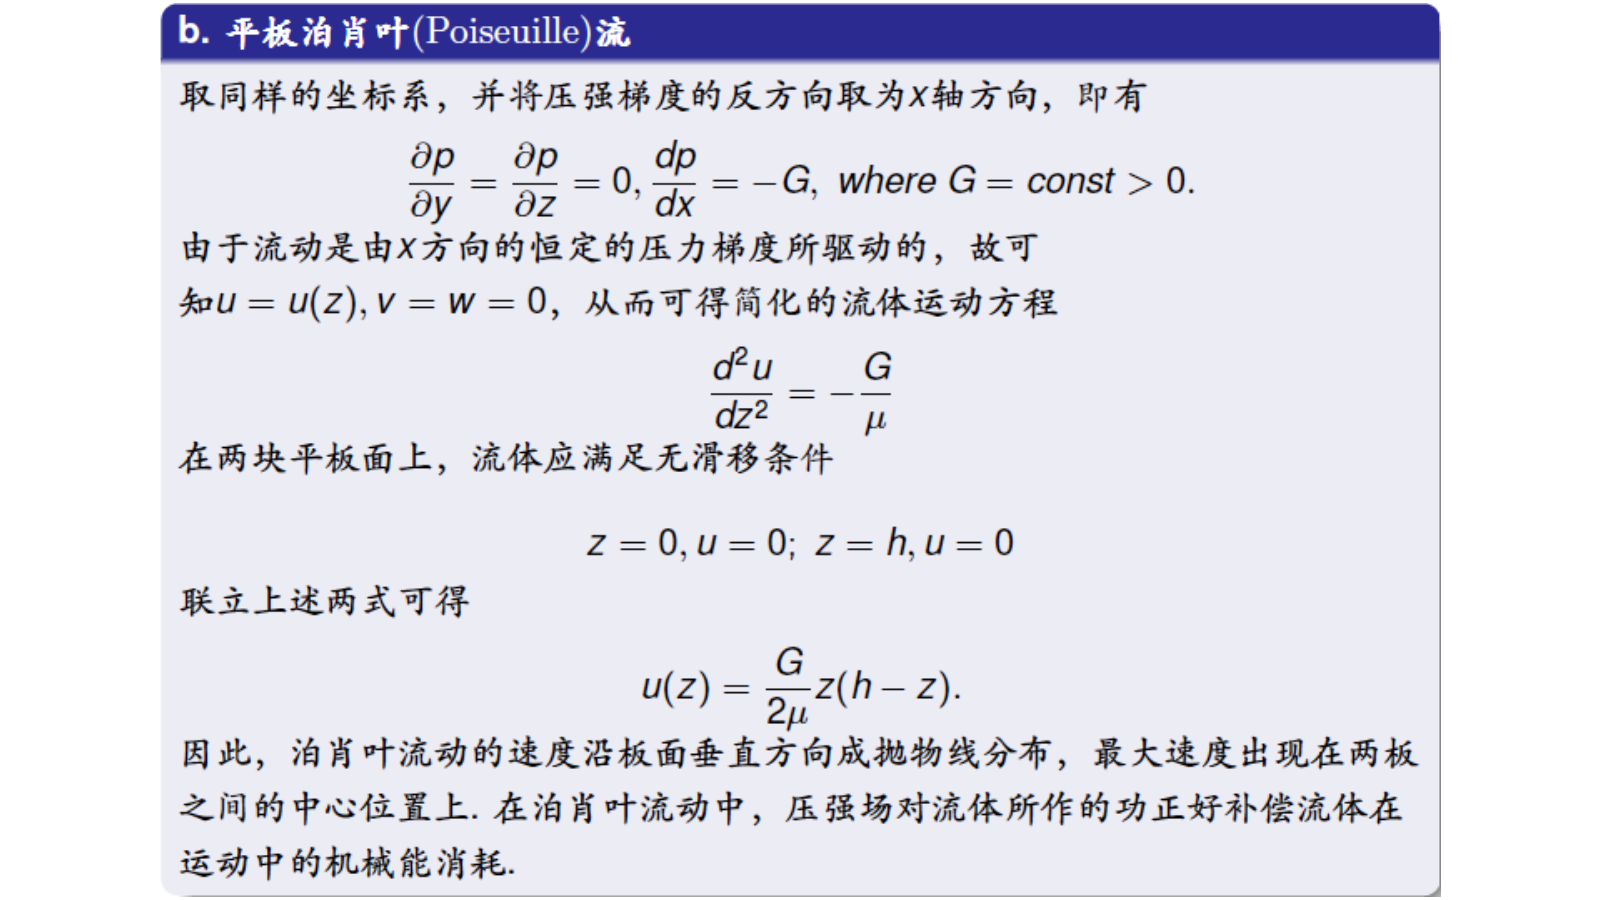
\includegraphics[width=.8\linewidth]{img/cal-2018_06_Page6.png}
\end{figure}

\begin{figure}[h]
    \centering
    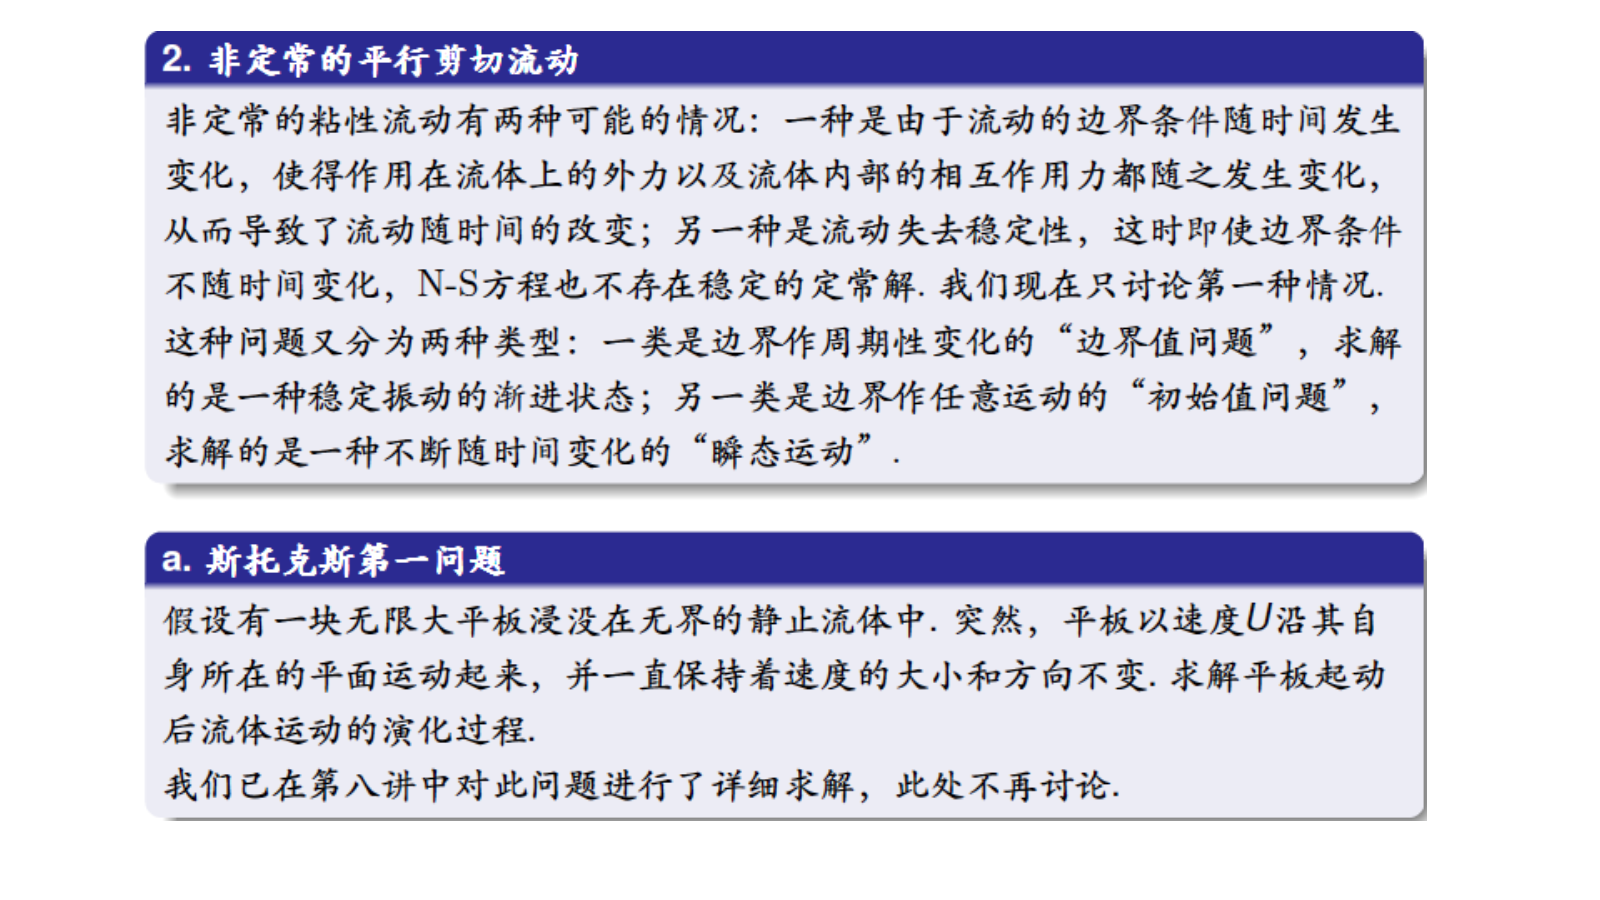
\includegraphics[width=.8\linewidth]{img/cal-2018_06_Page7.png}
    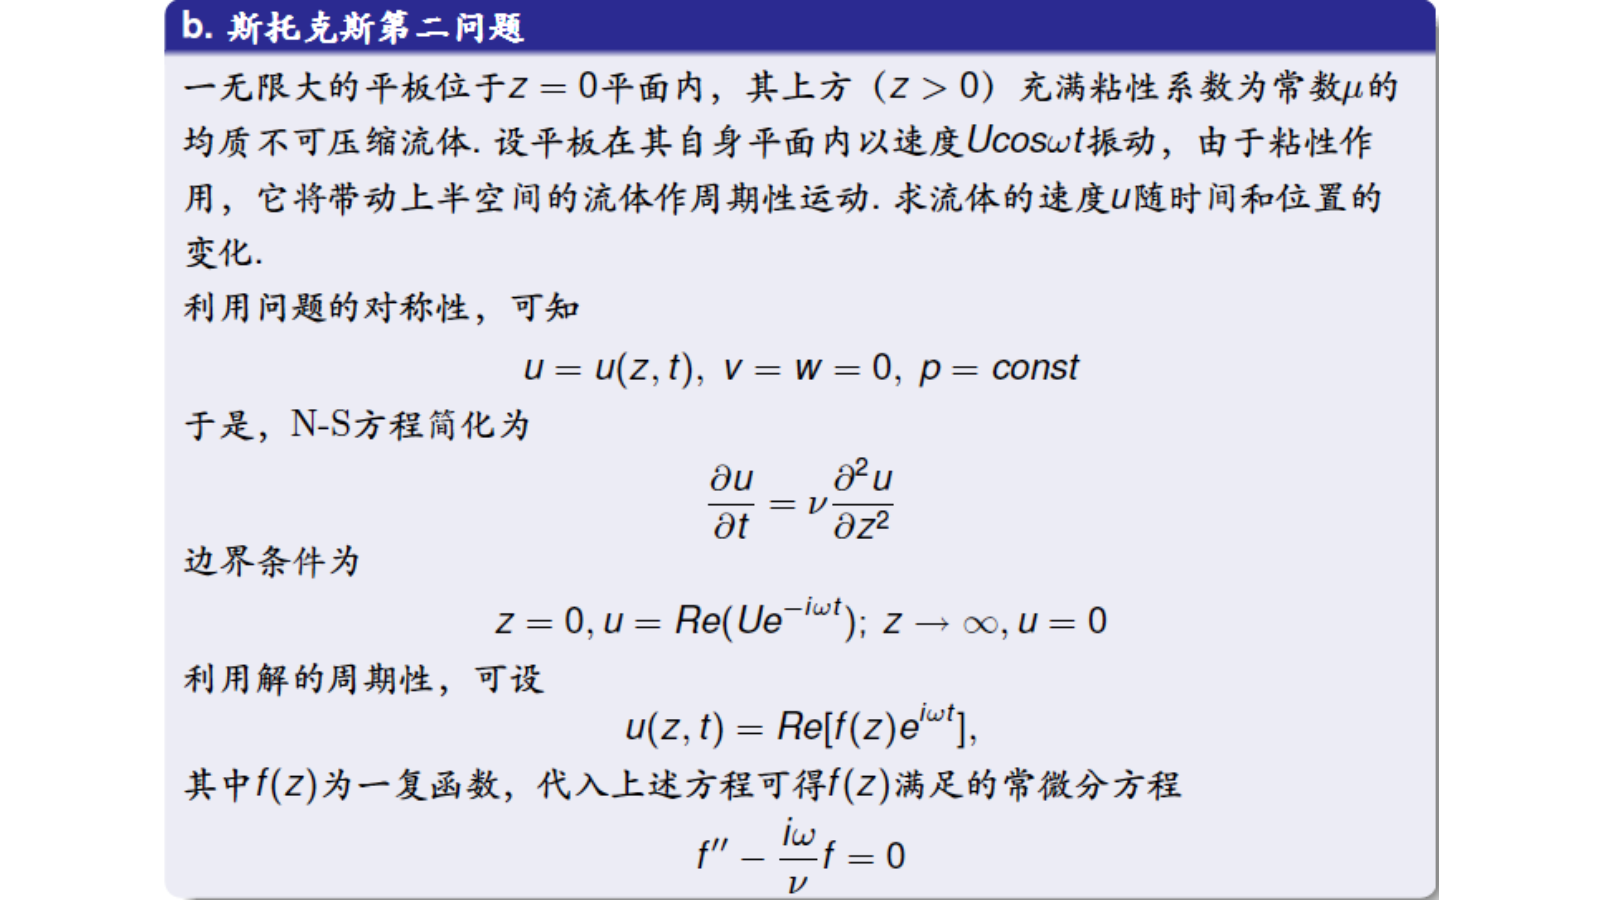
\includegraphics[width=.8\linewidth]{img/cal-2018_06_Page8.png}
    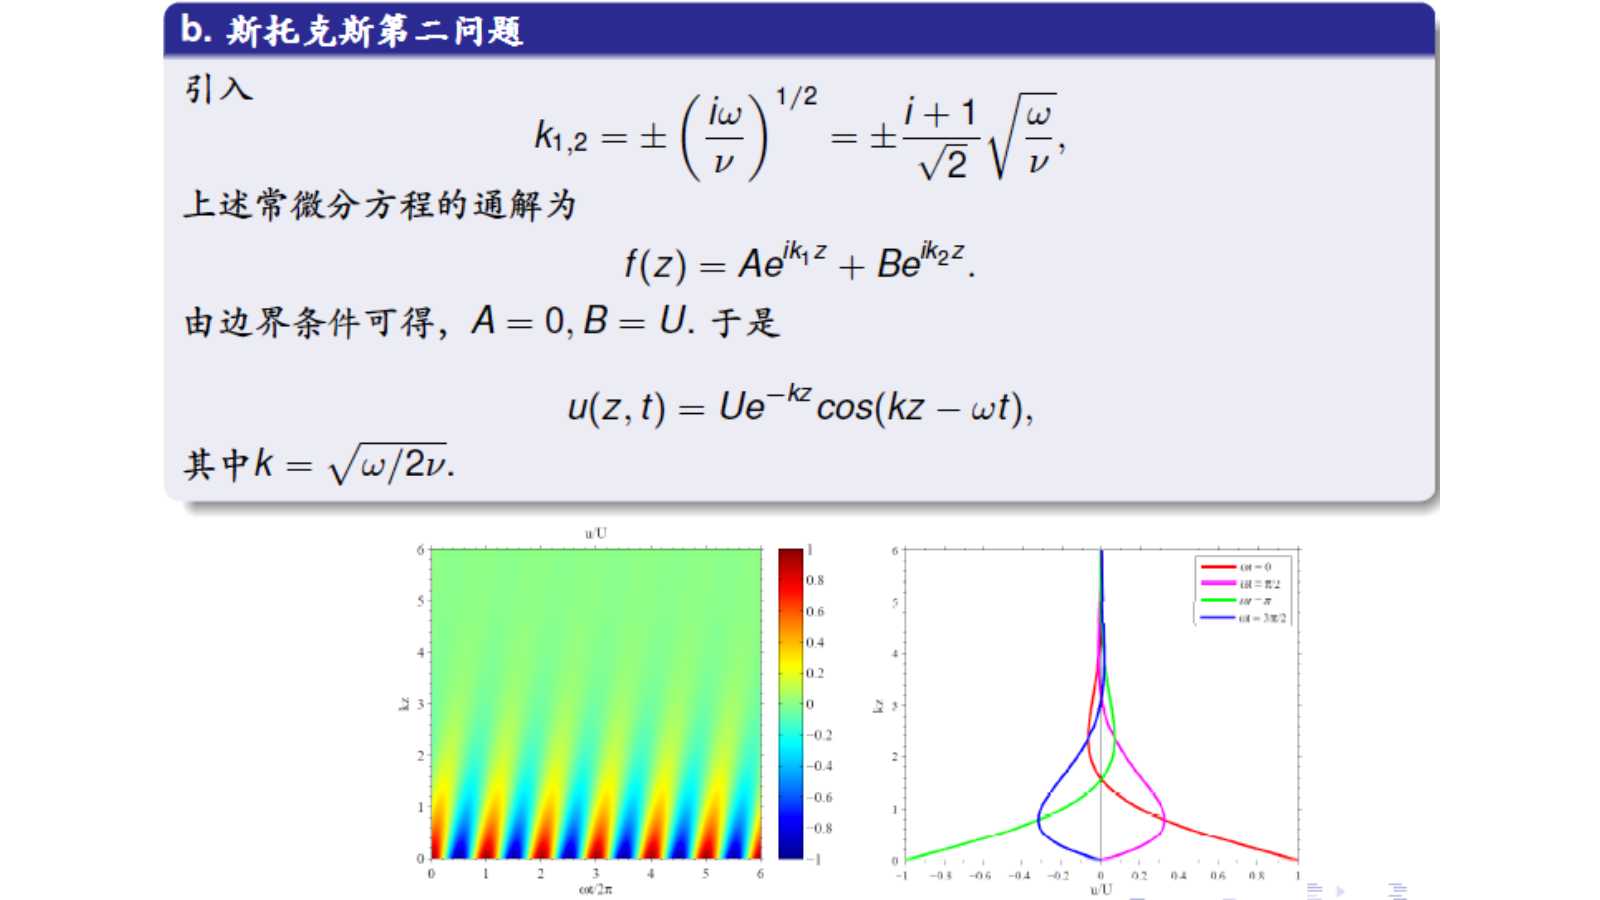
\includegraphics[width=.8\linewidth]{img/cal-2018_06_Page9.png}
%    \caption{Caption}
%    \label{fig:my_label}
\end{figure}

\section{Summary}

借这个机会,给这个学期(研究生第一学期)做个总结吧。之前老是觉得研究生挺远,应该和本科有很大不一样。现在读了一学期吧,发现确实不一样,又确实没什么变化。就还行。

这个流体力学,感觉还是下了功夫,最后还行吧,虽然最后一个课本例题的连续性方程没写出来。但是感觉流体力学学懂了。不仅仅是欧拉拉格朗日的互换、描述的意义,流线迹线的意义,最重要的是一些基本概念,比如偏导(随体导数那里)、偏导变化的原因,最后的粘性无粘的数学物理方程的求解。感觉本科期间很大的一个遗憾得到了填满。其实懂了也就很简单,就是把NS方程写出三个方向的分量,然后进一步简化,水平方向上是否有体积力、压强梯度力还是得看题目本身。然后就是简单的ODE,哈哈哈哈说不定本科那时的数学物理方程也就这样子吧。

行啦,这份资料有不少错别字,懒得修改啦,江湖路远,还会再见的。

\end{document}